
\chapter{Tuning the Surface Chemical Potential in Bi$_2$Te$_2$Se by Ionic Liquid Gating Method\label{ch:liquid}}

As we have discussed in previous chapters, it is of great practical value to increase the surface contribution in TI's conductance. Besides, there are many theoretical proposals such as building Chern insulators based on TIs, which require a chemical potential to be at the Dirac point. Thus it needs us to tune the chemical potential into the bulk band gap and close to the surface Dirac point. As a result, there has been a great amount of work trying to tune the chemical potential in TIs\cite{Checkelsky_gating, PabloBi2Se3, SacepeGate, PabloFilm, FuhrerBi2Se3, Checkelsky_liquid, IwasaMBE, Ando_liquid}.

Typically there are two methods to tune the chemical potential. One is to use the chemical doping method and one is to leverage a gating technique. Since there are few states (including the impurity states) inside the band gap, the chemical doping method may cause a large change in the carrier density and it is easy for the chemical potential to move across the band gap. Besides, the dopants introduce extra defects that can act as scattering centers and decrease the mobility of the sample. Therefore, it is favorable to use the gating method to fine tune the chemical potential in TI samples. 

Several groups\cite{Checkelsky_gating, PabloBi2Se3, SacepeGate, PabloFilm} have used the solid-state gating method to tune the chemical potential in different TIs. In many of these experiments, the quantum oscillations from the surface states on TIs are absent or very tiny, possibly due to the damage on the surface during the lithography process. Therefore the surface contribution in these samples is neither large nor of high quality, and the properties of the surface Dirac electrons at different $E_F$ remain to be explored.

Together with our group, some groups\cite{Yuan2011, FuhrerBi2Se3, Checkelsky_liquid, IwasaMBE, Ando_liquid} started to use another novel gating method, i.e. ionic liquid gating, to tune the chemical potential in TI crystals. Ionic liquid is composed of free-moving cations and anions. Hence, when a sample is immersed inside the ionic liquid and an electric voltage is applied, ions inside the liquid will move and one type of ions will pack on the surface of the sample and generate a large electric field on the sample surface. Besides, when the liquid is cooled down and becomes a solid, the ions are frozen and stay at the same position, maintaining the same electric field on the sample. Also, since the thickness of the ion layer on the sample is on the atomic scale, the electric field is very large and thus it can change the carrier density by a large amount. Such a powerful gating effect has been proved on many different materials, such as ZnO\cite{yuan2009ZnO}, ZrNCl\cite{ye2010liquid} and MoS$_2$\cite{YeMoS2}. We will show our results on tuning the surface chemical potential on Bi$_2$Te$_2$Se with the ionic liquid in this chapter.

% include other files for sections of this chapter. These use the 'input' command since each section within a chapter should not start a new page.
% If you want to swap the order of sections, it is as simple as reversing the order you include them. 
\section{Ionic Liquid Gating Experiments on Topological Insulators}
\label{sec:liquid:gating}

\subsection{Background and Introduction}

As explained in the above chapters, Bi$_2$Te$_2$Se has one of the most insulating bulk among all the Bi-based topological compounds, and its high-mobility surface state has been detected by quantum oscillations in transport experiments even at a temperature as high as 38 K~\cite{Xiong2012}. However, the surface chemical potential $E_F$ in our as-grown Bi$_2$Te$_2$Se crystals is persistently quite high ($\sim$200 meV above the Dirac Point), despite the large amount of effort that we have taken to bring down the chemical potential by the chemical doping method. Since the chemical doping method often changes the carrier density by a large amount, the chemical potential is easily tuned outside the bulk band gap. Furthermore, it is common that different segments of the as-grown Bi-based TI crystals have different $E_F$, adding the difficulty in the transport study. Thus it is desirable to tune the $E_F$ by an \emph{in-situ} gating method in order to explore the Dirac point. 

%Many groups have applied conventional electrostatic gating to tune the chemical potential $E_F$ both in exfoliated crystals~\cite{Check11,Pablo,Morpurgo} and in thin-film samples of Bi$_2$Se$_3$.~\cite{Steinberg}. Also, almost simultaneously with us, some groups started to leverage the newer technique, namely liquid gating method, to change the $E_F$ of Bi-based materials~\cite{Iwasa,Fuhrer,Check12,Iwasa12,Ando12}. These groups have shown a powerful gating ability on TI that the ionic liquid could have. However, in those work, the crucial surface quantum oscillations were absent, and the properties of the surface Dirac electrons at different $E_F$ remain to be explored.

%In our experiment, we immerse the 50um thick Bi$_2$Te$_2$Se samples with the gold-wired contacts in the ionic liquid DEME-TFSI, comprised of cations (CH$_3$ CH$_2$ )$_2$ (CH$_2$ CH$_2$ OCH$_3$ )CH$_3$ N+ and anions (CF$_3$SO$_2$)$_2$N?. The crystal dimensions of Sample 1 are 0.9?0.75? 0.05 mm$^3$. For Sample 2, they are 1.35 ? 0.61 ? 0.026 mm$^3$. The liquid is first pumped at $25 \,^{\circ}{\rm C}$ for 2 h prior to application in order to minimize any water content. Then the sample, the ionic liquid and the gold gate plate are put into a sapphire container, and are quickly loaded into the cryostat. Then the sample is fast cooled down to around 220K to reduce any chemical reaction or damage that could happen to the sample before the liquid freezes. After the gate voltage $V_G$ is applied to the gold plate at a �gating temperature� around 220K(see below), the sample is cooled to 4 K slowly (at 2K/min) to reduce the stress on the sample caused by the freezing ionic liquid. At 4 K, the large $E$-field induced by the frozen surface anion density $N_{ion}$ (1-4$\times 10^{14}$ cm$^{-2}$) creates a depletion layer that penetrates deep into the bulk (5-20 $\mu$m) (We will provide the analysis in later sections). As shown in Fig. \ref{figRRH}b (inset), the induced upward bending of the bands decreases $E_F$.This cooling process has a possibility to damage the sample as we find that repeated freezing and thawing of the ionic liquid can snap the leads or the crystal itself. Also, a large |$V_G$| may trigger an electrical discharge which invariably leads to a steep collapse of R (at 5 K).
%
%Unlike in thin films, changes to the resistance of our bulk samples caused by |$V_G$| are not resolved above ?100 K [see Fig. \ref{figRRH}], possibly due to their thickness and large amount of thermally activated carriers at high temperatures. As previous ionic liquid gating experiments (citations), every time we change $V_G$, we need to warm up the sample to the "gating temperature" around 220K and change $V_G$ by small steps. At the "gating temperature", a typical way to change $V_G$ is to change it in steps of ?0.02 V, while monitoring the transient current $I_trans$ (1-40 nA). The time spent at the "gating temperature" is typically 300�500 s, as we will discuss later in this chapter. Then the sample is cooled down to 5K slowly with the gating voltage fixed. To minimize the sample damage, we start at $V_G$ = 0 during the first cool-down, followed by measurements at increasingly negative $V_G$ until the sample fails (usually by a discharge event).  We emphasize that the changes to ? and nH are reversible (see below) as long as |$V_G$| does not exceed a limit. Upon returning $V_G$ to 0, we could recover the same starting value of R (at 5 K) provided |$V_G$|  is kept below 2 V.

%%%%%%%%%%%%%%%%%%%%%%%%%%%%%%%%%%
%%%%%%%%%%%%%%%%%%%%%%%%%%%%%%%%%%
%%%%%%%%%%%%%%%%%%%%%%%%%%%%%%%%%% FIGURE 1

%%%%%%%%%%%%%%%%%%%%%%


In this chapter, we will discuss our ionic liquid gating experiments on Bi$_2$Te$_2$Se. We observed prominent Shubnikov-de Haas oscillations in our magneto-resistance measurement at various gating voltages. Our results show that the periods of  the surface SdH oscillations can be changed over a broad range by an ionic liquid called DEME-TFSI. We find that ionic liquid could reduce $E_F$ by 50\% and we are able to access the $N$ = 1 Landau level in a magnetic field $B$ = 14 T. It allows us to investigate Bi$_2$Te$_2$Se's $\pi$ Berry phase with greatly improved resolution, as the $\frac12$-shift in the index plot remains fixed when the surface chemical potential is brought down by 50\%. More importantly, one surprising finding is that our ionic liquid gating method enhanced the surface mobility $\mu_s$ by three times according to our enlarged quantum oscillations. A possible explanation is the "smoothing" of the local potential fluctuations that increase the scattering of the surface electrons. The ionic liquid gating method provides us an opportunity to explore the direct information of both the bulk and surface with different chemical potentials, such as how the surface and bulk mobilities change with the gate voltage $V_G$. 

To fully understand the change of the surface and bulk carrier densities as well as the band bending effect in our gating experiment, we also combine the inferred parameters from the quantum oscillations and a semiclassical two-band model to explain Bi$_2$Te$_2$Se's Hall signals under different gating voltages. From the clear and large SdH oscillation data, we can obtain five transport parameters at each $V_G$, including the chemical potential $E_F$ and the mobility $\mu_s$ of the surface carriers, the bulk density and mobility, and the total ionic charge Q deposited on the surface of the sample. These five parameters together provide us a comprehensive and detailed picture of our gating experiments and the band-bending model. Also, since the parameters inferred from the SdH oscillations typically have very small error bars, such test greatly reduces the possibility for misunderstanding the experimental data. Through these analysis, we could also determine the depletion capacitance C$_d$ as well, which measures the polarizability of the depletion region.


%Despite the strong gate tuning ability of ionic liquid, there is some debate on whether the change of $E_F$ is caused by its large capacitance or by chemical reactions. To fully understand the mechanism behind, we discuss our evidence that the liquid gating in our experiment is inducing band bending rather than unwanted chemical reaction. 
\subsection{Experimental Details}





%The crystal dimensions of Sample 1 are 0.9?0.75? 0.05 mm$^3$. For Sample 2, they are 1.35 ? 0.61 ? 0.026 mm$^3$. In Sample 2, the steepest change in ?s occurs between $V_G$ = 0 and $V_G$ =?1.5V,at which $\mu_s$ =2800 $cm^2/Vs$.At a larger gate, it saturates ($\mu_s$ = 3000 $cm^2/Vs$ at ?6 V).

In our gating experiments, we follow the steps introduced in the previous chapter ``Experimental Setup'' to tune the gating voltages, and are able to change the sample's longitudinal and Hall resistance by a significant amount. The change of the sample resistance can be seen clearly in the resistance-temperature curves as displayed in Fig. \ref{figRRH}. As reported earlier~\cite{Ando10,Xiong2012,Xiong2012b}, the resistance $R(T)$ of $n$-type as-grown Bi$_2$Te$_2$Se rises dramatically to very large values as $T\to$ 4 K (curve at $V_G$ = 0 in Fig. \ref{figRRH}a). As a negative $V_G$ is added to the sample, the 4 K resistance increases as $|V_G|$ becomes larger, and eventually is enhanced by 40$\%$ at the most negative $V_G$ (Fig. \ref{figRRH}a). Previous work on the Hall coefficient has shown that at 5 K the population of bulk $n$-type carriers is much higher than the population of surface electrons (Fig. \ref{figRRH}b). Through the ionic liquid gating, the Hall coefficient $|R_H|$ increases by a factor of 2 at 5 K (Panel b) at the largest $|V_G|$. But at $|V_G| >$ 3 V both R and $R_H$ saturate, as expected for the ionic liquid gating experiments\cite{Yuan2011}. Previous work shows that chemical reactions start to happen at these voltages\cite{Yuan2011}. The change in both the resistance and the Hall coefficient at different $V_G$ suggests an upward bending of the bands and a decrease of $E_F$ at negative $V_G$ as long as $V_G$ does not exceed the depletion limit.

%The chemical doping to the sample in a strong $\bf E$ field is an an important concern in liquid-gating experiments. 

\begin{figure}[!htbp]
  \begin{center}
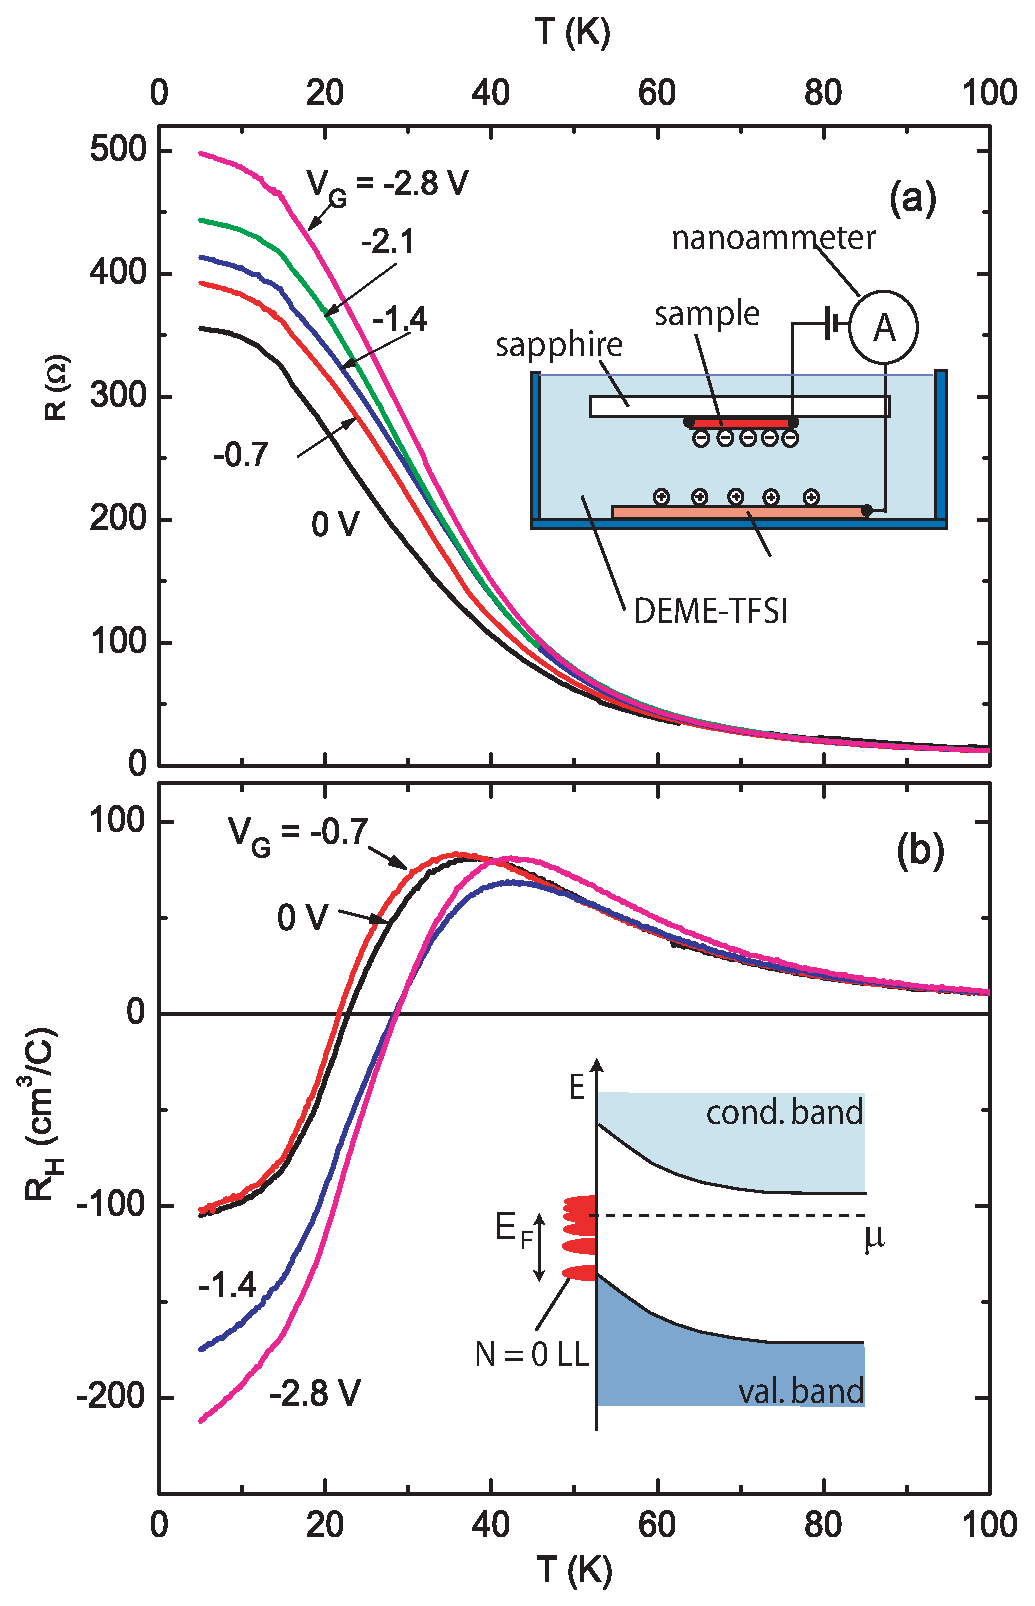
\includegraphics[width=0.75\linewidth]{ch-liquid/figures/FigRR.eps}
\caption{\label{figRRH} The resistance $R$ per square (Panel a) and
Hall coefficient $R_H$ vs. $T$ (Panel b) in Bi$_2$Te$_2$Se at selected $V_G$ in Sample 1. 
$R_H$ is measured at fixed $B$ (3 T) using the reciprocal method in Ref. \cite{Sample1987}. When $V_G$ is changed from 0 to -2.8 V, $R$ increases by 40$\%$ and $|R_H|$ increases by 2$\times$ around 5 K. The inset (Panel a) shows 
the cell housing the sample and the ionic liquid DEME-TFSI. The Au gate electrode (a
circular plate of radius 1.5 mm) is separated by 0.5 mm from the sample.
The inset in (b) is a sketch of the band bending induced by liquid gating. 
Negative ions deposited on the crystal leads to upward band-bending and a decrease of surface chemical potential towards the Dirac point. Landau levels formed by the surface electrons are shown as solid half-ovals.
}
  \end{center}
\end{figure}


Though the ionic liquid appears to have a strong power to change the carrier density in the sample, there is a debate about whether such a change is caused by its large capacitance or by certain chemical reactions. To investigate this issue, we set up some measurement in which $V_G$ is reversed, as we will discuss in the appendix. Briefly speaking, we notice that any changes caused by chemical reactions are inherently nonreversible. It means that if the chemical doping is the main reason for the changes in $\rho$ and $n_H$ at finite $V_G$, then the values of $\rho$ and $n_H$ should not return to their starting values by resetting $V_G$ to 0 V, as the chemical damage to the sample could not be recovered. And we can examine such changes at 4 K as the changes in $\rho$ and $n_H$ are most distinct at 4K. Therefore, by cycling $V_G$ we will be able to tell whether severe chemical doping has happened to the sample or not. If the band bending is the dominant effect in our gating experiment and chemical reaction effects are minimal, there will be no hystereses in $\rho$ and $n_H$ (measured at 4 K) as $V_G$ is cycled. Otherwise, we should be able to notice a large hysteresis. Thus we need to test the absence of resolvable hystereses in $\rho$ and $n_H$ when cycling the gating voltages. In addition, the test can tell us the voltage limit under which the chemical reactions can be neglected. We will show the results of such tests in the appendix. To introduce it briefly, we performed many tests on Sample 3 to investigate details of the ion accumulation in the $V_G$ cycling process over a broad range of gating temperatures (208 $<$ T $<$ 260 K). We have not performed these tests on Samples 1 and 2, from which the detailed SdH results were obtained, as we hope to minimize stress damage to their surfaces.

\begin{figure}[!htbp]
  \begin{center}
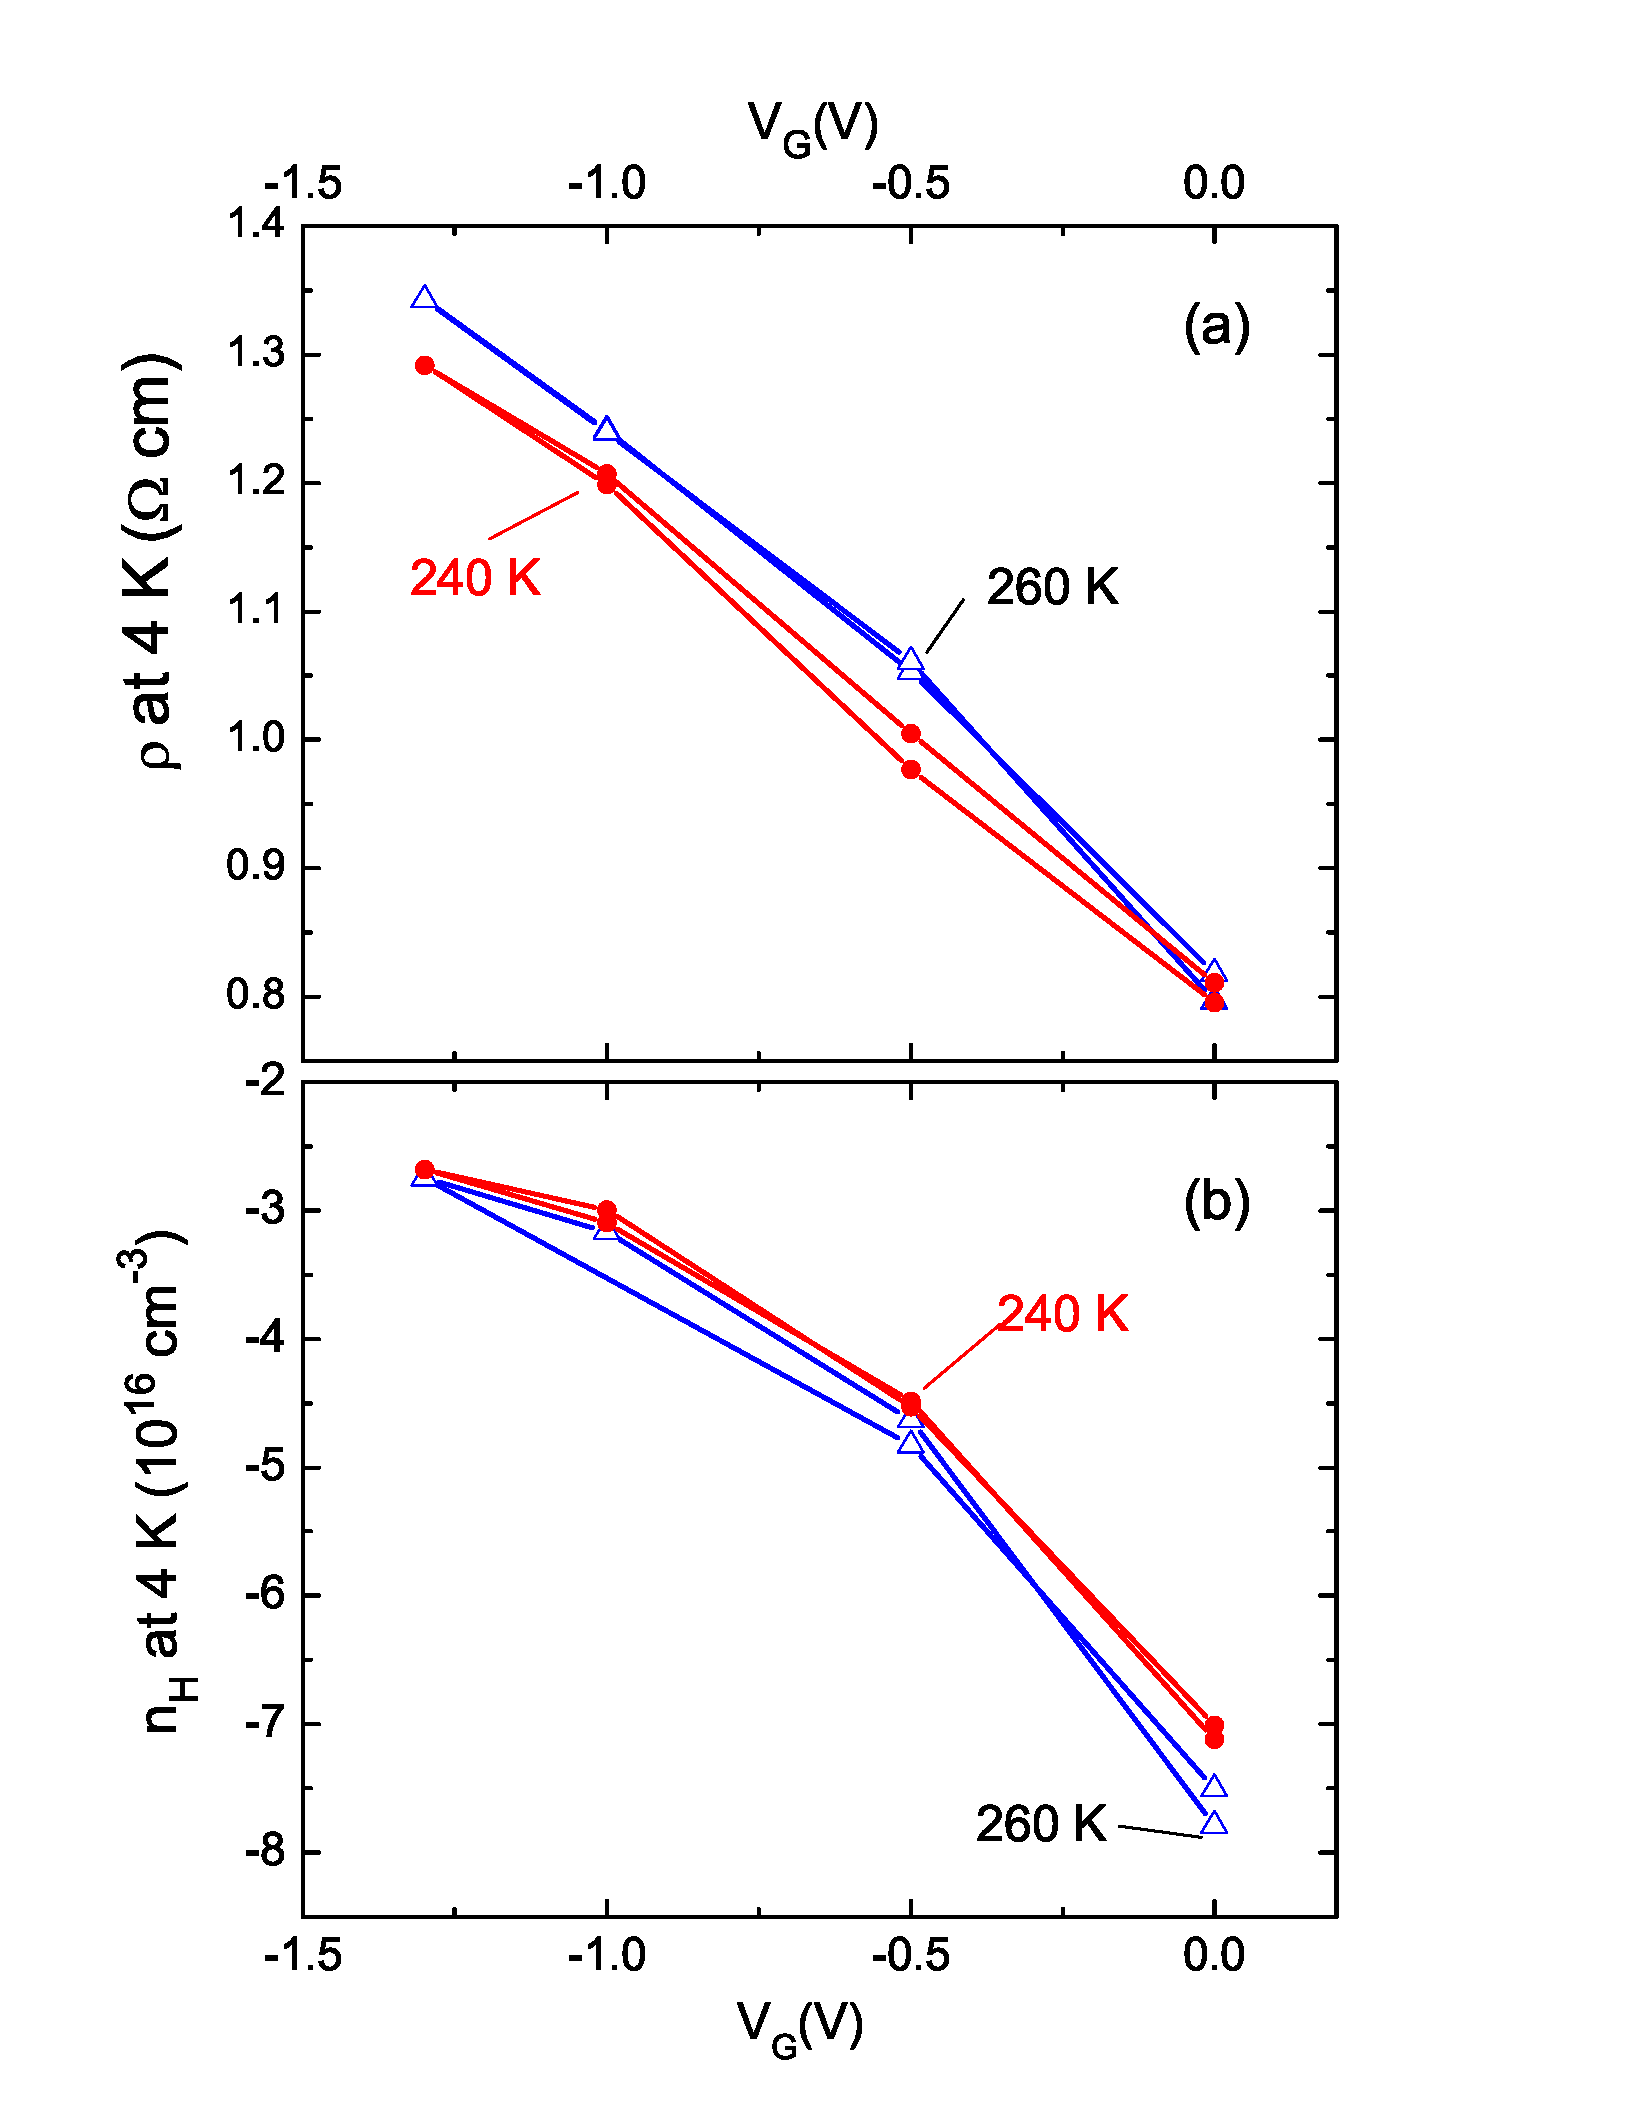
\includegraphics[width=0.75\linewidth]{ch-liquid/figures/FigRvsVG.eps}
\caption{\label{RvsVG} 
Test experiments to show negligible hysteresis in the sample�s resistivity $\rho$ (a) and Hall density $n_H$ (b), as $V_G$ is changed from 0 to -1.3 V, then back to 0 V at temperatures T = 240 and 260 K (Sample 3). The small hysteresis (within the measurement uncertainties) is taken as evidence that the chemical reaction is negligible compared with the physical gating effect. The accumulation time is 800 s in order to collect all the charge.
}
  \end{center}
\end{figure}


Fig. \ref{RvsVG} shows the main result of the $V_G$ cycling experiment on Sample 3. $V_G$ is changed stepwise from 0 to $-$1.3 V and back, while both $\rho$ and $n_H$ at 4 K are monitored at each step. Here $V_G$ is set anew (at the gating T = 240 K and 260 K respectively), and we wait for 800 s to accumulate all the anions before cooling to 4 K for the measurements of $\rho$ and $n_H$. During the change of $V_G$ at 240 K, we also record the transient charging current $I_{trans}$ in order to test whether the accumulated charges are fully reversible and hence cause the band-bending effects. As shown in Fig. \ref{RvsVG}, both at the gating temperature of 240 K and 260 K, $\rho$ and $n_H$ show clear variations at different $V_G$, but they have negligible hysteresis.


Apart from chemical reaction, two other important factors are incomplete melting of the ionic charge configuration when T is too close to the glass transition and the intrinsic (activated) bulk conductance of the ionic liquid. We have investigated these additional factors by measuring the charge accumulation during the $V_G$ change. We discuss them in the appendix. The detailed discussion about the choice of gating temperatures will also be in the appendix.

 
%\begin{figure}[htb]
%  \begin{center}
%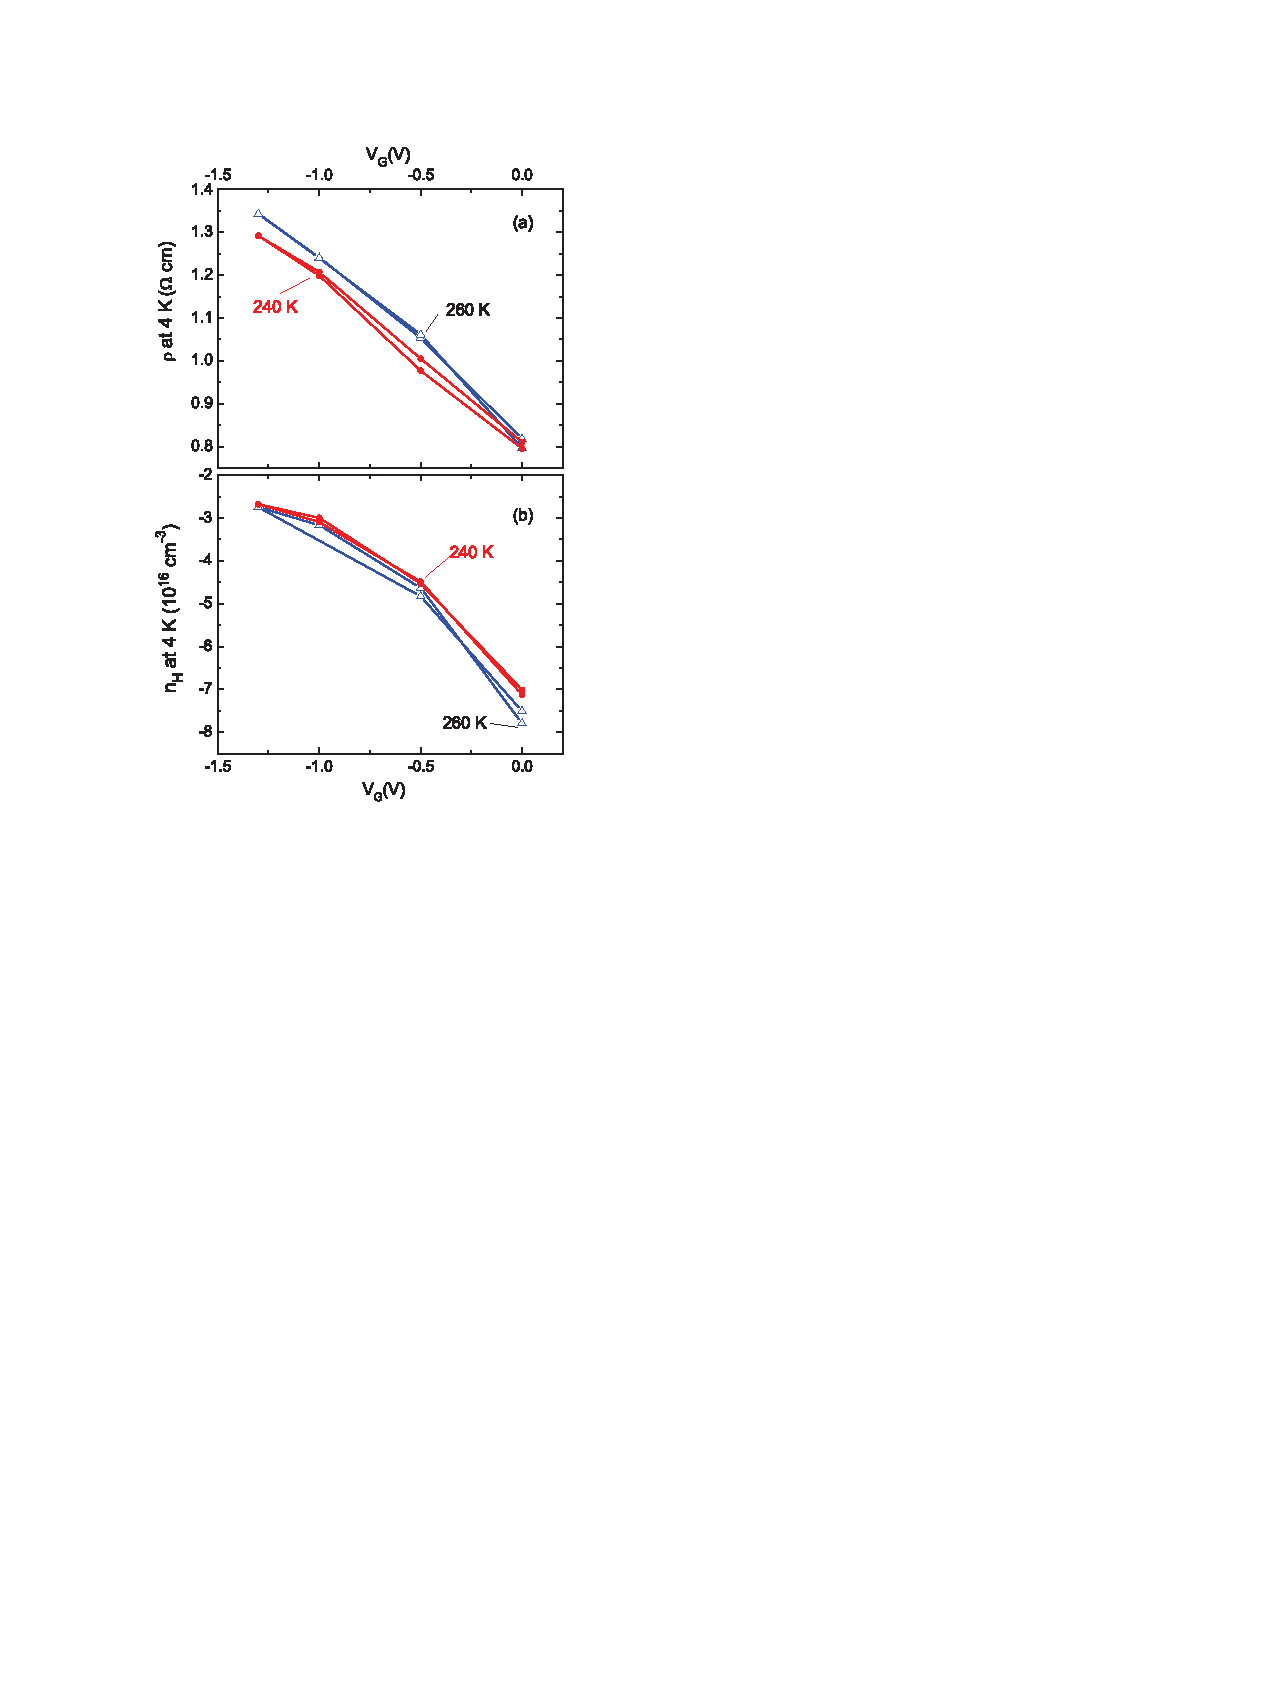
\includegraphics[width=0.9\linewidth]{ch-liquid/figures/nVg.pdf}
%\caption{\label{fignVg} (color online)
%Test experiments
%  \end{center}
%\end{figure} 

%%%%%%%%%%%%%%%%%%%%%%%%%%%%%%%%%%
%%%%%%%%%%%%%%%%%%%%%%%%%%%%%%%%%%
%%%%%%%%%%%%%%%%%%%%%%%%%%%%%%%%%% FIGURE 2


\subsection{Quantum Oscillations in Magnetoresistance under Different $V_G$}

\begin{figure}[!htbp]
  \begin{center}
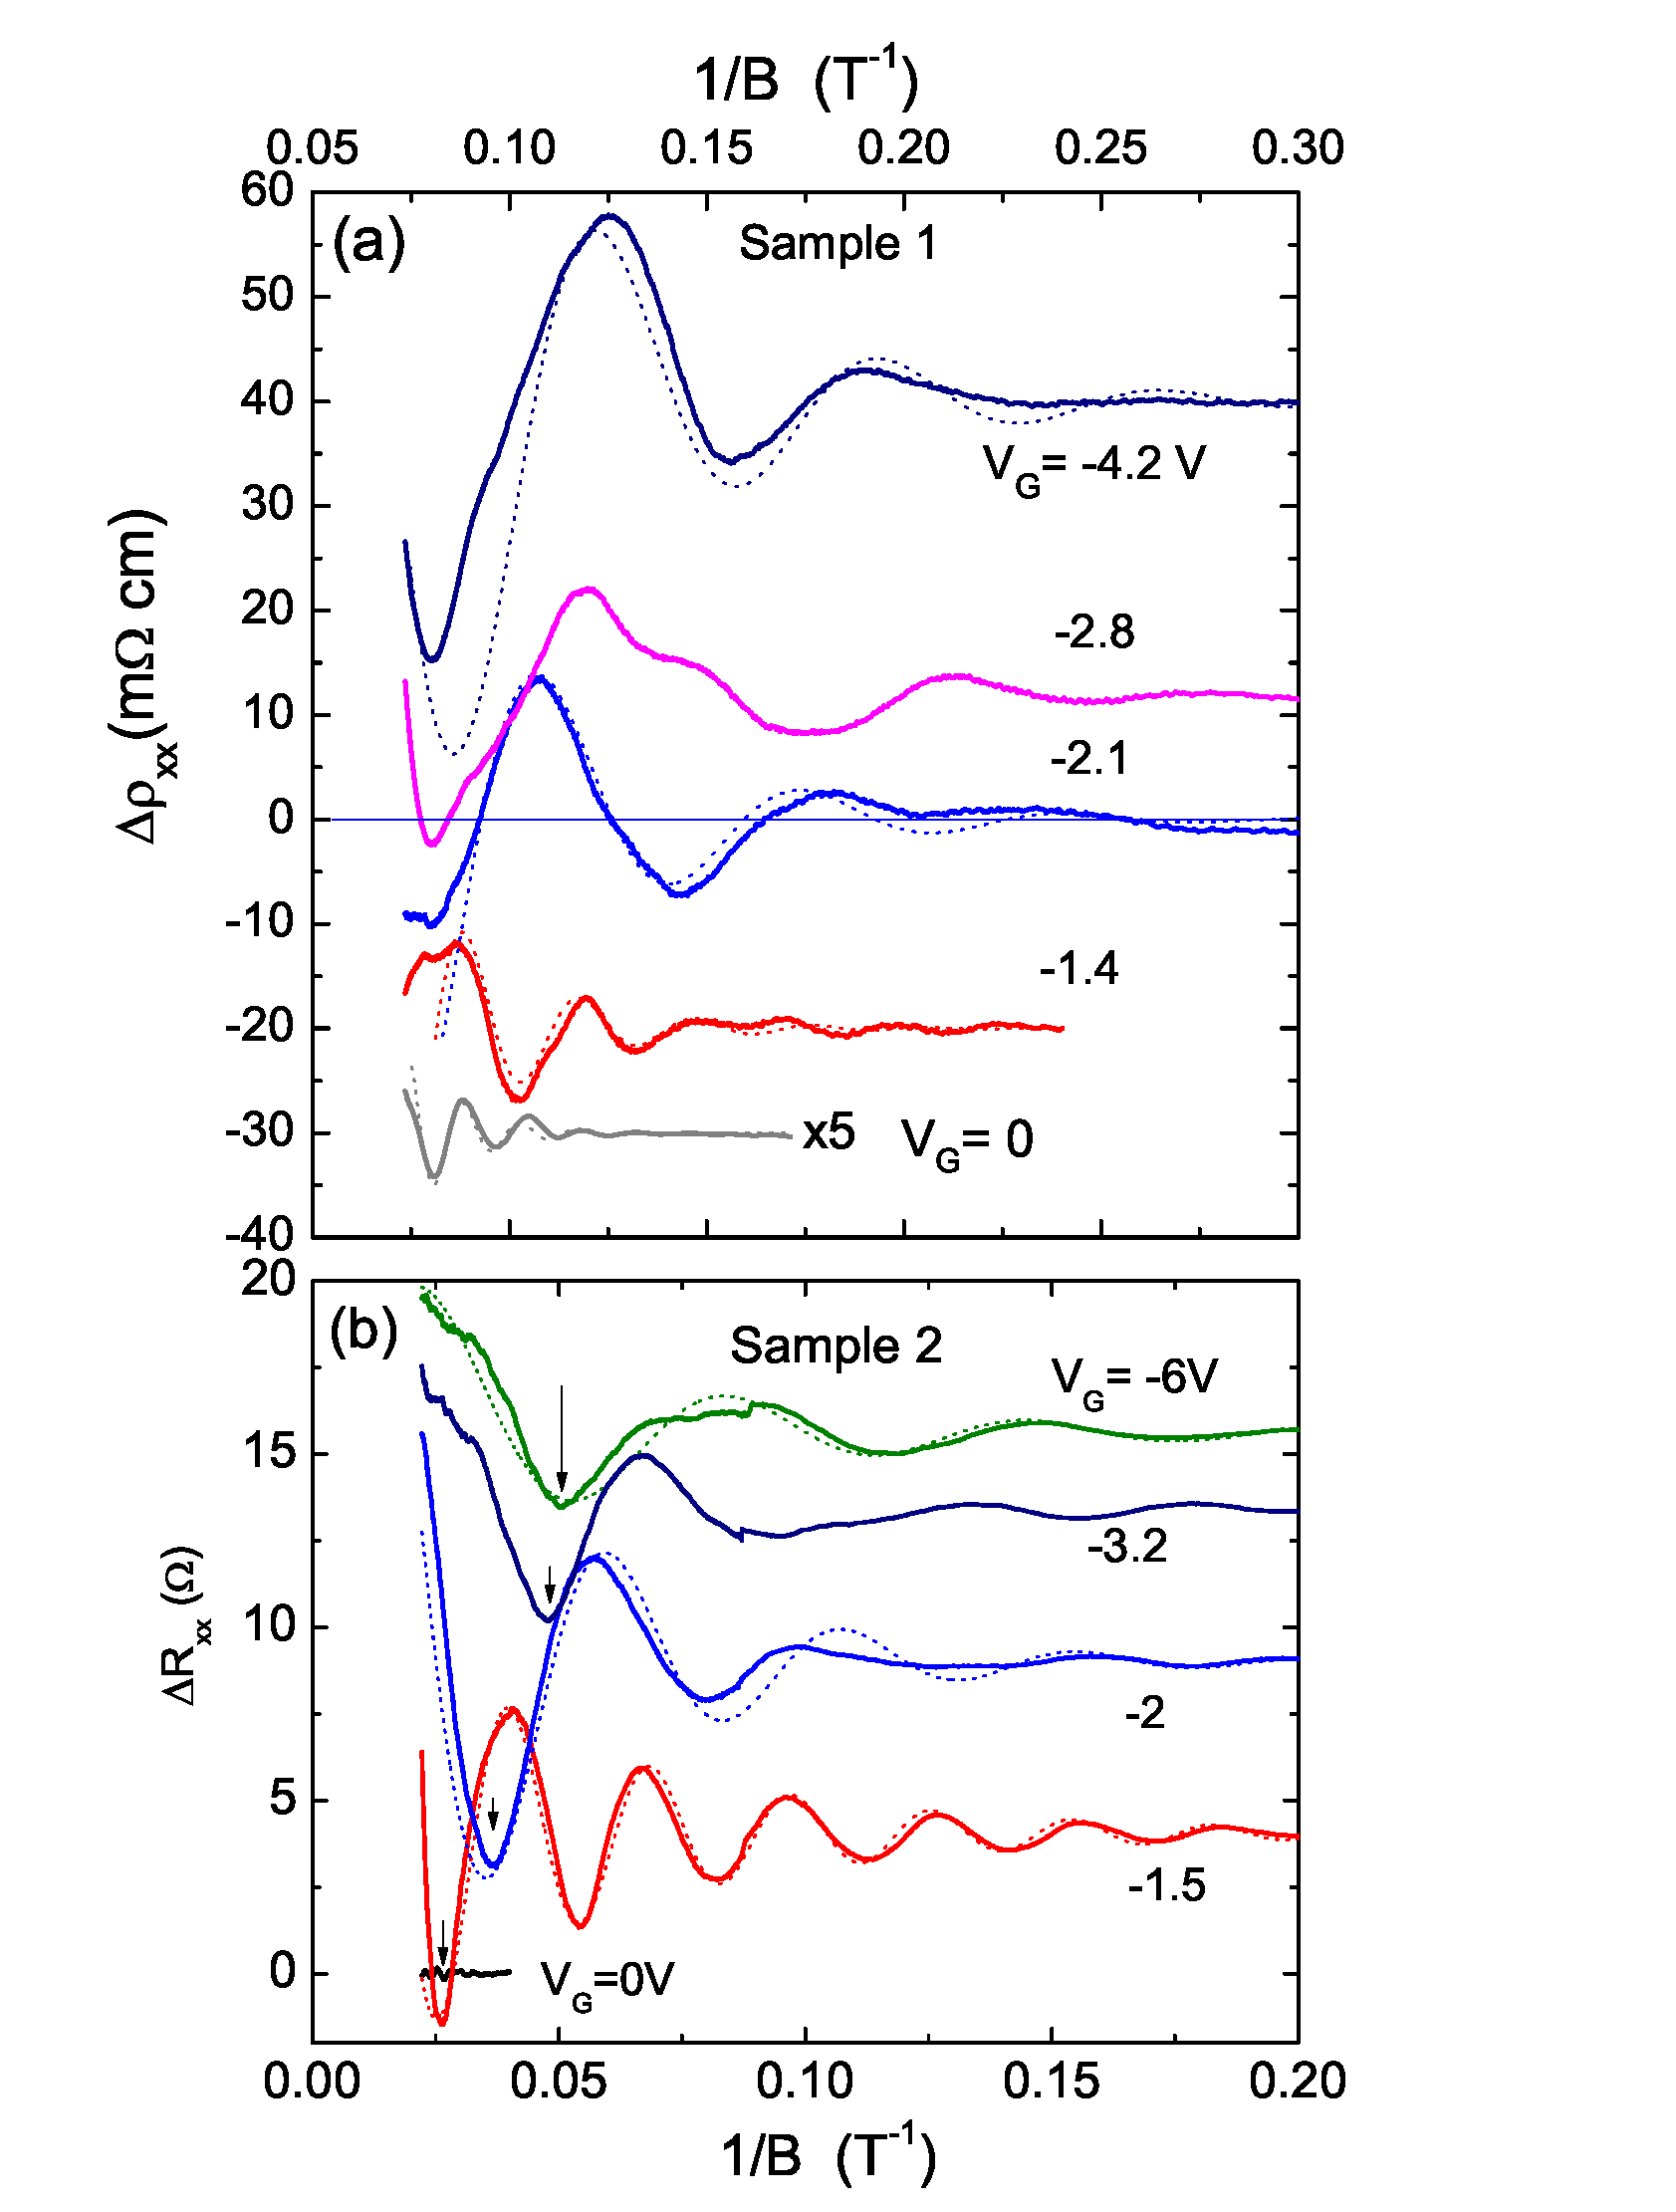
\includegraphics[width=0.85\linewidth]{ch-liquid/figures/FigSdHAll}
\caption{\label{figSdH_Vg}
Traces of SdH oscillations in the resistance versus $1/B$ curves of Sample 1 and 2,
showing systematic changes in the oscillation amplitudes and periods as the gate voltages increase
(bold curves, displaced vertically for clarity). The dashed curves
are fits to the LK expression with one frequency component~\cite{Xiong2012b}. 
Panel (a) shows traces of $\Delta\rho_{xx}$ 
vs. $1/B$ at 5 K measured up to 14 T for 5 values of $V_G$ (Sample 1). 
The largest increase in amplitudes occurs between $V_G$ = 0 V and -1.4 V. The curve
at $V_G = 0 V$ is shown after an amplification of $5\times$. All other curves share 
the same vertical scale. Panel (b) displays traces of $\Delta R_{xx}$ vs. $1/B$ at 0.3 K 
measured up to 45 T at $V_G$ as indicated (Sample 2).
Arrows indicate $n=\frac12$ ($E_F$ at center of broadened $N$ = 1 LL). 
}
  \end{center}
\end{figure} 

At each $V_G$, the magnetoresistance curves for both Sample 1 and 2 display giant SdH oscillations. In Fig. \ref{figSdH_Vg} we have subtracted a smooth background $\rho_B$ from the raw data to emphasize the SdH oscillatory part of the resistance. Therefore, the oscillatory part is $\Delta \rho_{xx} \equiv \rho_{xx} - \rho_{B}$, where $\rho_{B}$ is a smooth background. Fig. \ref{figSdH_Vg}a displays plots of $\Delta\rho_{xx}$ v.s. $1/B$ in Sample 1 for 5 different gate voltages. The period of the SdH oscillations clearly has a large monotonic increase as $V_G$ changes from 0 to -4.2 V, indicating a decreasing $E_F$ of the $n$-type surface states as we expected. Unexpectedly, the SdH amplitudes are strongly enhanced between $V_G = 0$ and -2.1 V (to show the former oscillations in the figure, we have amplified its amplitudes by 5$\times$). The dotted curves are the best fits ~\cite{Xiong2012b} to the Lifshitz-Kosevich (LK) expression for SdH oscillations using only one frequency component. From the fits, we can infer how the surface mobility $\mu_s$ changes with $V_G$ (see below). We find the same trend in Sample 2, which has a higher starting surface density $n_s$ but is taken to $B$ = 45 T (Fig. \ref{figSdH_Vg}b). Although the SdH oscillations are not resolved at $V_G=0$ V, they become prominent starting at $V_G$ = -1.5 V. From the fittings, we also notice that the steepest change in $\mu_s$ of Sample 2 occurs between $V_G$ = 0 and $V_G$ =$-$1.5V, at which $\mu_s$ =2800 $cm^2/(Vs)$. At a larger gating voltage, it saturates ($\mu_s$ = 3000 $cm^2/(Vs)$ at $-$6 V) as the gating effect saturates. 





%%%%%%%%%%%%%%%%%%%%%%%%%%%%%%%%%%
%%%%%%%%%%%%%%%%%%%%%%%%%%%%%%%%%%
%%%%%%%%%%%%%%%%%%%%%%%%%%%%%%%%%% FIGURE 3




%%%%%%%%%%%%%%%%%%%%%%%%%%%%%%%%%%
%%%%%%%%%%%%%%%%%%%%%%%%%%%%%%%%%%
%%%%%%%%%%%%%%%%%%%%%%%%%%%%%%%%%% FIGURE 4




\section{Analysis of the Experimental Results}
\label{sec:liquid:analysis}

\subsection{Analysis of the Quantum Oscillations}
In a strong magnetic field perpendicular to the sample surface, the Dirac surface electrons are quantized into Landau levels (LLs) with quantum numbers $N = 0,1,\cdots$. Here we take the same definition of the index field $B_n$ as in Ref. \cite{Xiong2012b}, which is also the same as our previous chapters. Thus $B_n$ is the field at which $E_F$ falls between two LLs. This definition can also be naturally extended to the quantum Hall regime.
For Schr\"odinger states, the integer $n$ counts the number of 
occupied LLs (the highest filled LL has $N_{max} = n-1$ with the energy $E = (N_{max}+\frac12)\hbar \omega$, where $\omega$ is the cyclotron frequency). Using the level 
degeneracy $Be/h$ per spin, we then have $1/B_n = ne/(hn_s)$ 
($n_s$ is the surface density, $e$ the elemental charge and $h$ is Planck's constant). Thus the Landau index plot in Schr\"odinger case has a zero intercept.

The Dirac electrons have an extra $\frac12$ shift in their LLs as we have
$n+\frac12$ filled LLs when $B = B_n$ (now $N_{max} = n$).
The additional $\frac12$ derives from the $N=0$ LL due to the particle-hole symmetry, or equivalently, 
from the $\pi$-Berry phase intrinsic to each Dirac cone~\cite{Kim}. 
The relation between $1/B_n$ and $n$ is now 
$ 1/B_n = (n+\frac12)(e/h n_s)$ -- a straight line that 
intercepts the $n$-axis at $n = -\frac12$. 
As we discussed in previous chapters, $G_{xx}$ provides a reliable way to decide $B_n$ even when the bulk conductance contributes significantly. And it is a local minimum at $B_n$ for both Dirac and Schr\"odinger electrons. Therefore, we can leverage the difference in the intercepts to distinguish the Dirac electrons and the Schr\"odinger ones.

\begin{figure}[!htbp]
  \begin{center}
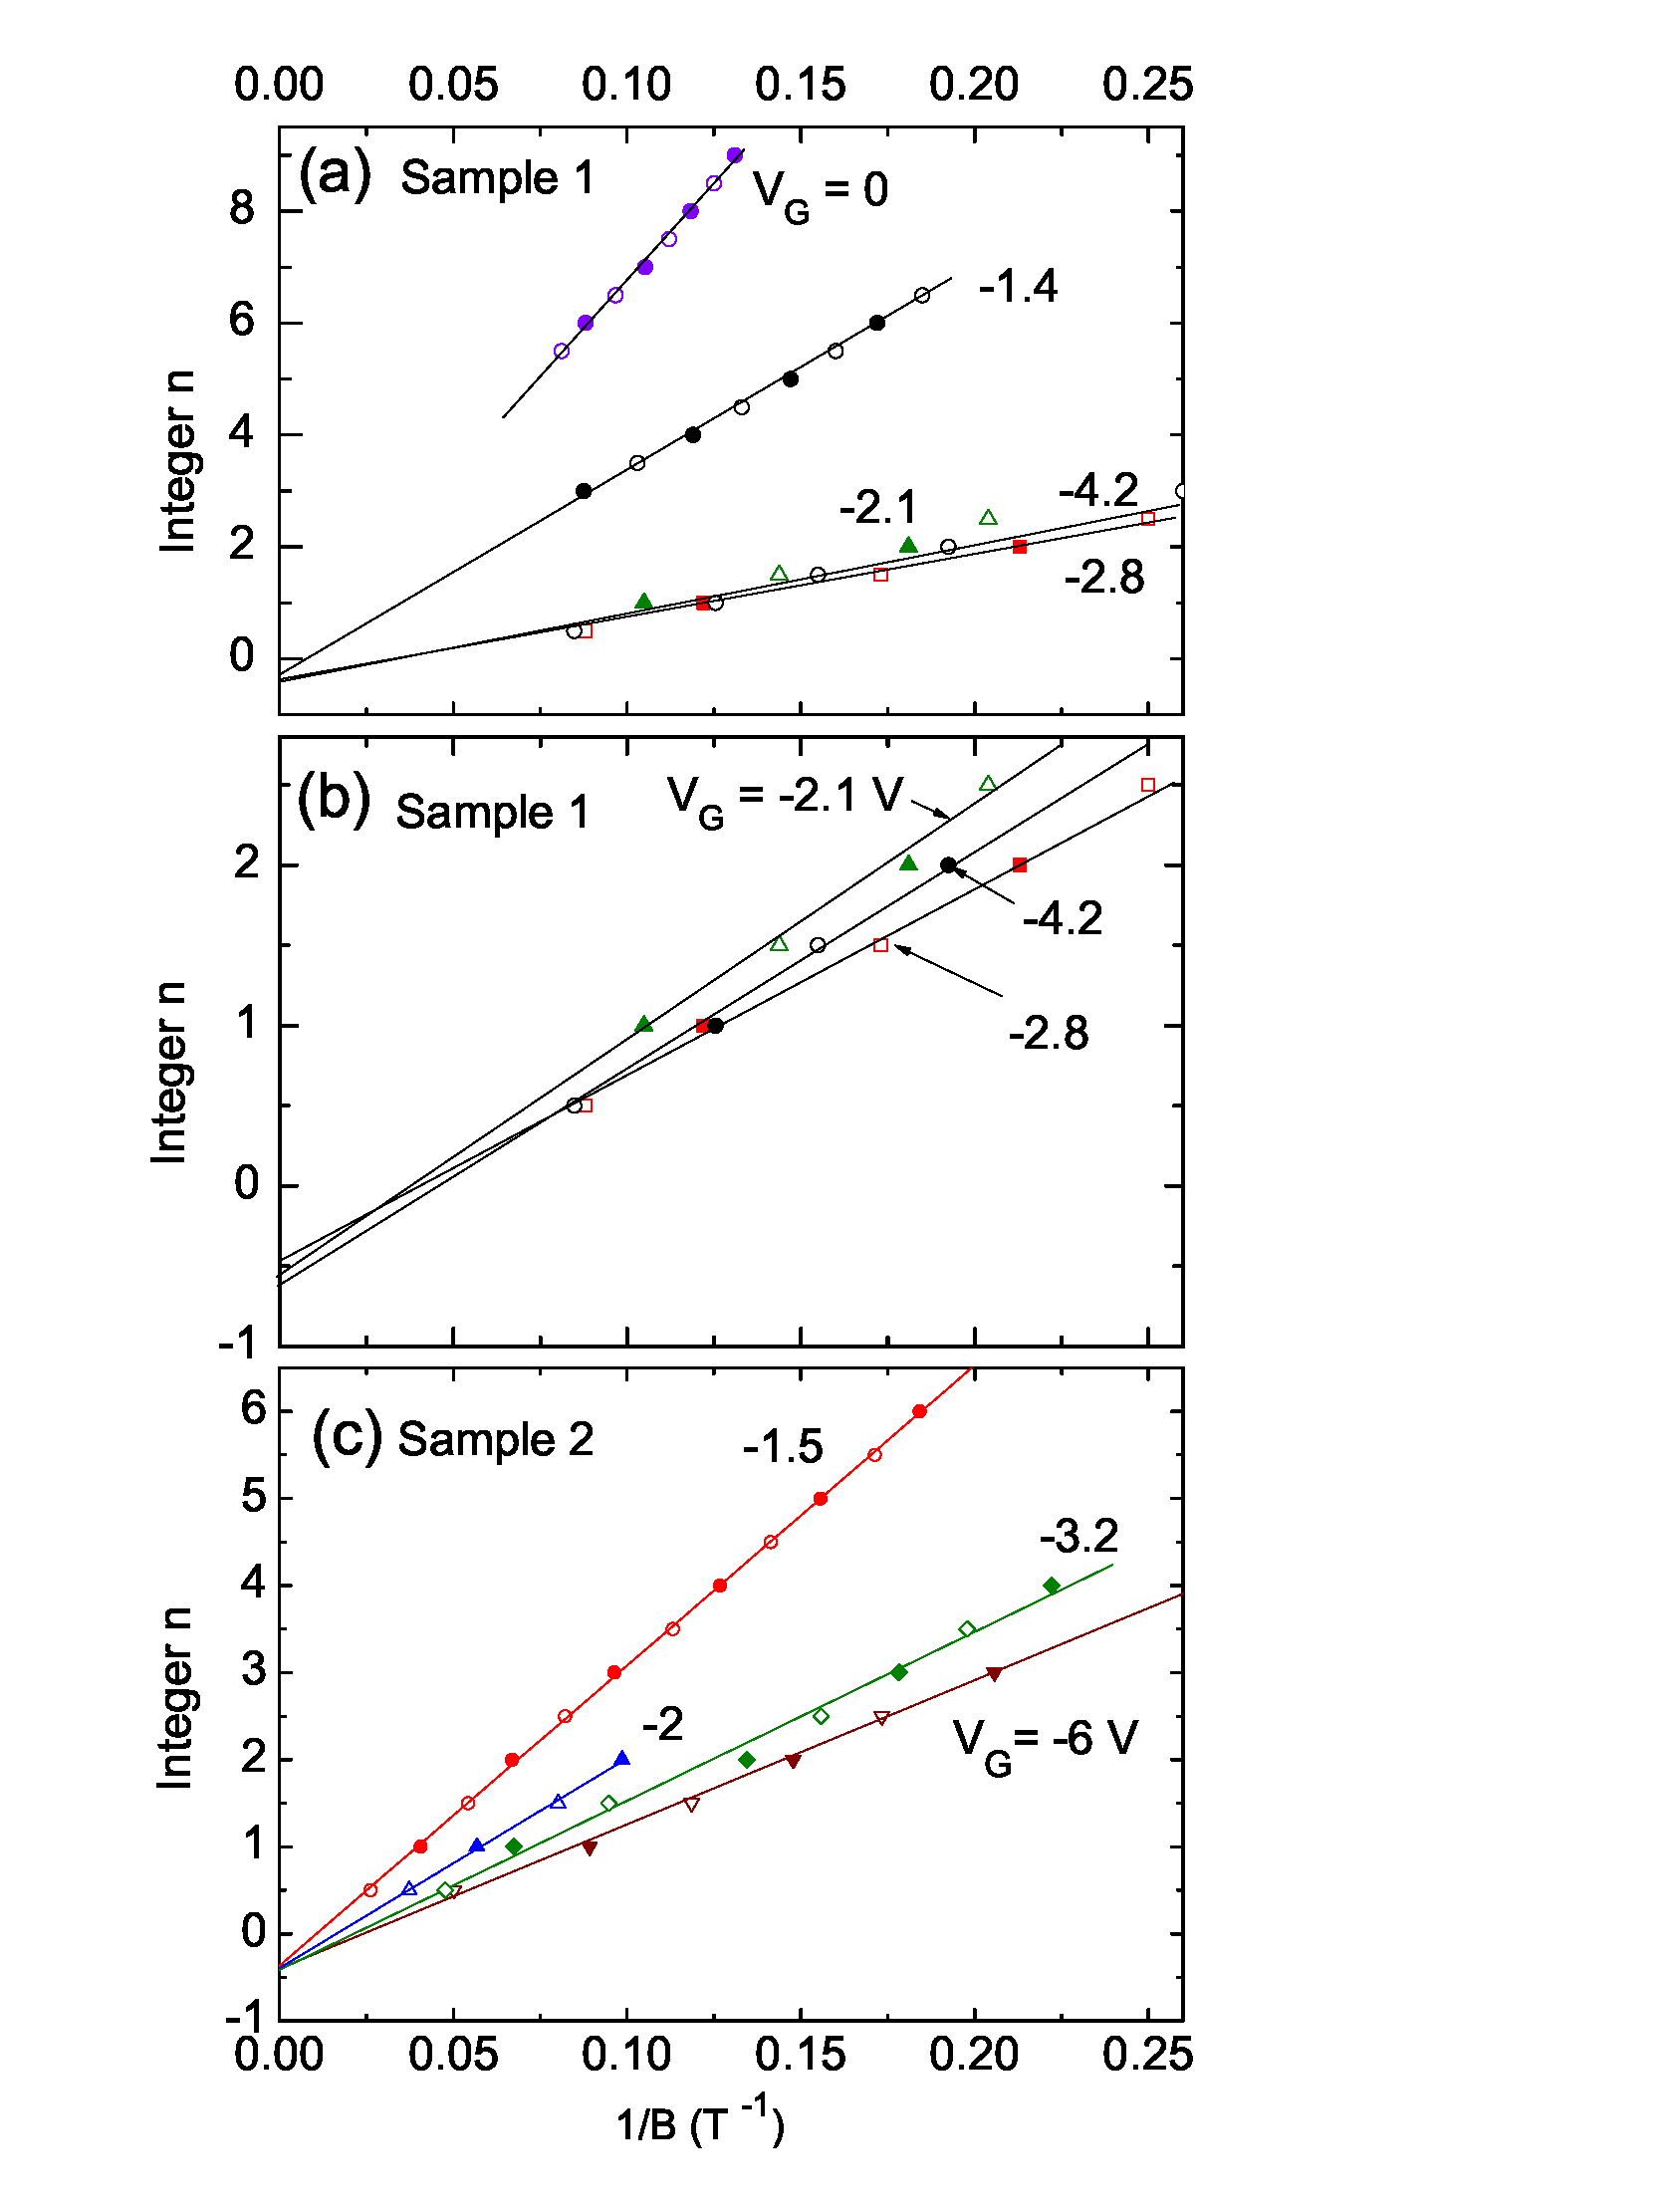
\includegraphics[width=0.85\linewidth]{ch-liquid/figures/FigIndexAll}
\caption{\label{figIndex} 
Index plots of the integer $n$ vs. $1/B_n$ at selected $V_G$ in Sample 1 (Panels a and b) and 2 (Panel c).
Maxima of $\Delta\rho_{xx}$ (solid symbols), corresponding to the index fields $B_n$, are plotted against $n$. Minima (open symbols)
are plotted against $n+\frac12$.
Panel (a): As $V_G$ changes from 0 to -2.1 V, the slope of the best fit lines decreases by six times, indicating a decrease of the carrier density by six times as well. Further increase
in $|V_G|$ leads to saturation of the slope. In Panel (b), the high-bias curves are displayed in expanded vertical scale to determine the intercept. In the limit $1/B\to 0$, the best-fit lines have intercepts at -0.46, -0.56 and -0.61 respectively for different $V_G$. They are close to $\frac12$ (mod 1), consistent with a Dirac dispersion.
The intercepts for Sample 2 (Panel c) also cluster near -0.45 in the limit $1/B\to 0$.
}
  \end{center}
\end{figure} 


However, if the resistivity curves are used to determine the Landau indices, $B_n$ should be identified with the \emph{maxima} in $\Delta\rho_{xx}$ as we discussed in the previous chapter. This is useful when the Hall data are not available. From the $\Delta\rho_{xx}$ v.s. $1/B$ curves in Fig. \ref{figSdH_Vg}, we plot as solid symbols $B_n$ in Sample 1 against the integers $n$ in Fig. \ref{figIndex}a
(the open symbols corresponding to the minima are plotted against $n+\frac12$). The straight lines in the figure are the least square fit to the index plots. The slopes of the fitted straight lines yield the Fermi surface area $S_F$ at different $V_G$. 
As $|V_G|$ increases from 0 to 2.8 V, the slopes of the best-fit lines 
decrease by a factor of 6.4, reflecting a steep decrease in $S_F$. 
This decrease saturates when $|V_G|$ exceeds 2.1 V. Such a decreasing $S_F$ at negative $V_G$ is expected as the anions on the sample surface deplete the $n$-type surface states.  

Then we leverage the intercepts of the fit lines to investigate the Dirac nature of the surface states at different $V_G$. As discussed in previous chapters, sometimes the slope of the index plot changes from the low field regime to the high field part. And the intercepts are fixed by the high field indices. Therefore, we show the high-field behavior for $|V_G|>$ 2.1 V in expanded scale in Panel (b) to obtain a higher accuracy in determining the intercepts. At various large bias values, the intercepts all gather around $n = -\frac12$ 
(-0.46, -0.56 and -0.61) for Sample 1. 

In the Landau index plot for Sample 2 (Panel c), we find that $S_F$ decreases by a factor
of 2 between $V_G$ = -1.4 and -6 V. In the limit $1/B\to 0$, the intercepts are at
$n= -0.35$, -0.40 and -0.42.  These values are all significantly closer to $-\frac12$ than 0 or 1.
The lowest index we obtain at the highest $B$ in both samples is $n_{min}=\frac12$, indicating that $E_F$ lies in the middle of the broadened $N=1$ Dirac LL. As we argued in the previous chapter, such a small $n_{min}$ is important for us to reduce the uncertainties and rigorously exclude an intercept at $n=0$ in the limit $1/B\to 0$. We illustrate the uncertainties incurred in Fig. \ref{figIndexError}a. At $V_G$=0 V, where the LL index is high, the uncertainties $\delta B_n$ in determining the index fields are typically $\pm5\%$ (circles). As shown, it could lead to a considerable spread in the allowed intercepts as we extrapolate the fitted line to the n-axis (the lowest datum corresponds to n = 5.5). By comparison, at the gate voltage $V_G$ = -2.8 V 
(squares), the lowest index is n = 1. This significantly reduces the spread in the allowed intercepts. The same advantage may be achieved by applying an intense $\bf B$ up to 45 T, as done in Ref. \cite{Xiong2012b}.
Therefore, by showing the $-\frac12$ intercepts at different $V_G$, we have provided more conclusive evidence for the Dirac and surface nature of the SdH oscillations on top of our previous discussions.

\begin{figure}[!htbp]
  \begin{center}
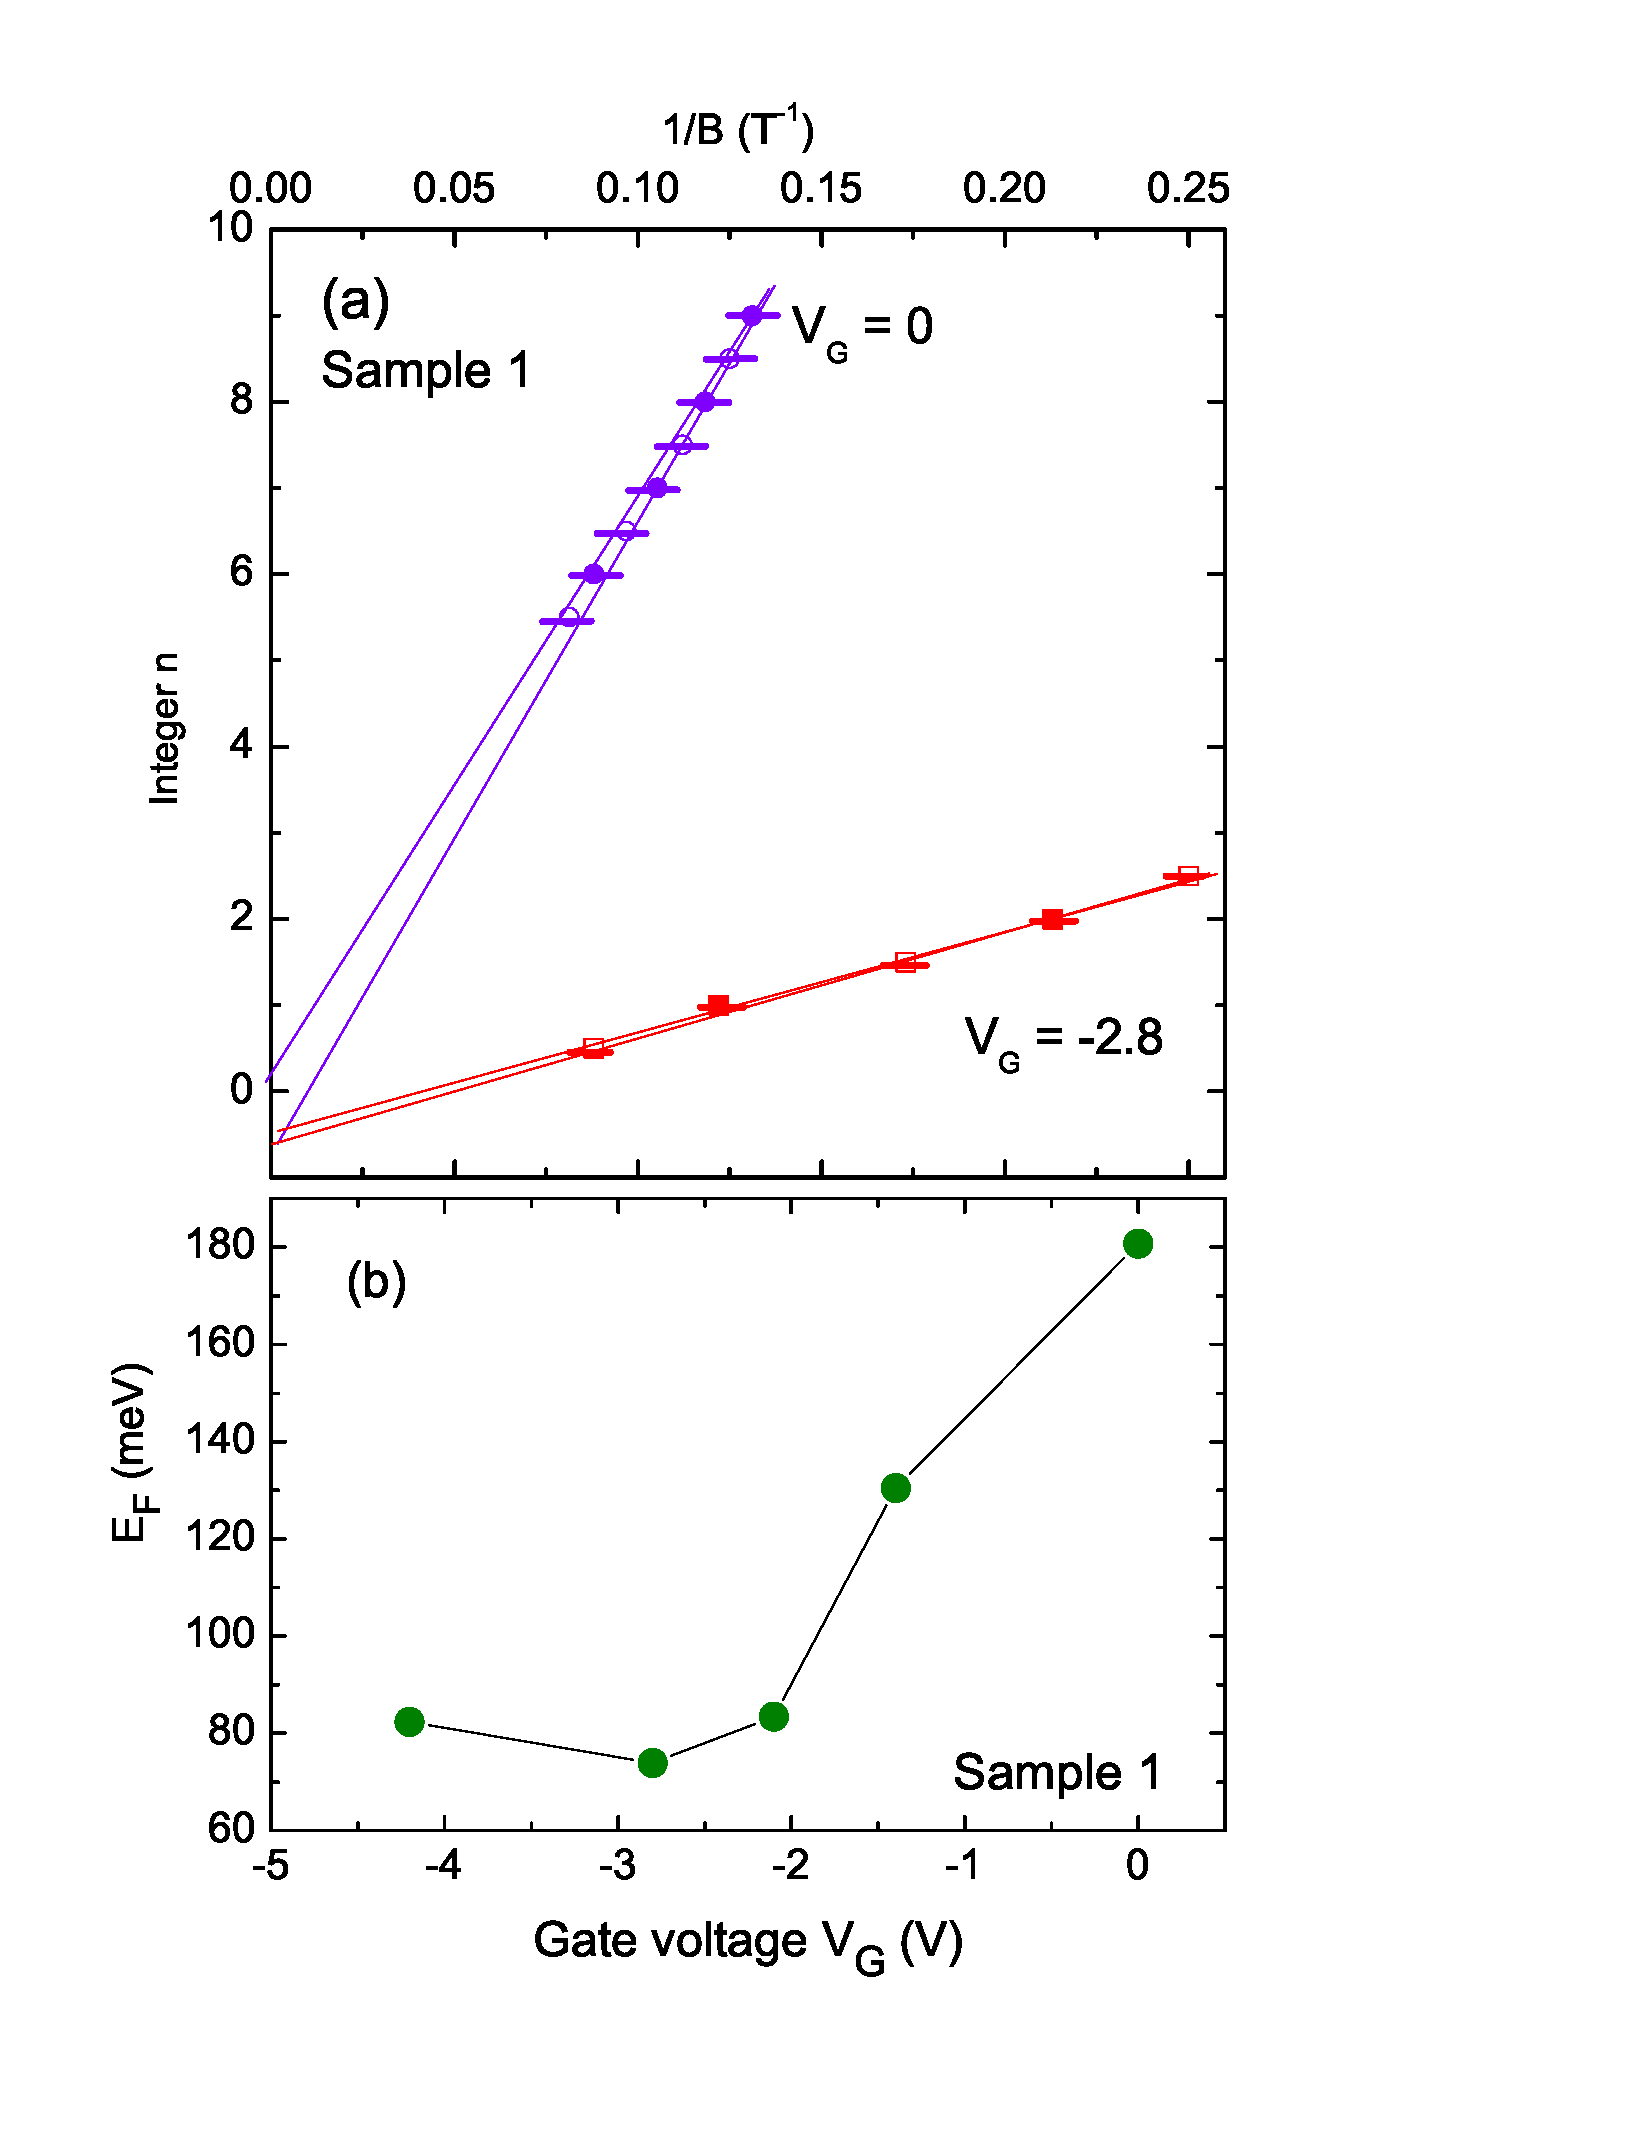
\includegraphics[width=0.85\linewidth]{ch-liquid/figures/FigIndexError.eps}
\caption{\label{figIndexError} 
Comparisons of extrapolations of the index plot to the limit $1/B \to 0$ for index fields measured with $V_G$ = 0 (circles) and measured with $V_G$ = -2.8 V (squares) in sample 1. (b) Variation of $E_F$ with applied $V_G$ in sample 1 ($E_F$ is measured from the Dirac point). The FS cross-section $S_F$ is converted to $E_F$ by $E_F = \hbar v\sqrt{S_F/\pi}$ 
using $v$ = 6$\times 10^5$ m/s~\cite{Xiong2012}. For $|V_G|> 2 V$, the decrease in $E_F$ saturates.
} 
  \end{center}
\end{figure} 


We also calculated the Fermi energy by $E_F=\hbar v \sqrt{S_F/ \pi}$ at different $V_G$, where $S_F$ is inferred from the slopes of the index plots in Figs. \ref{figIndex}. The Fermi velocity we use here is $v_F = 6 * 10^5 m/s$~\cite{Xiong2012}. Fig. \ref{figIndexError}(b) shows that $E_F$ in Sample 1 has been dramatically reduced from 180 meV to around 80 meV when $V_G$ changes from 0 V to -2 V. Thereafter, it remains at $\sim80$ emV at large $|V_G|$. Below we also use this information to estimate the depletion capacitance. Another thing we notice is that $E_F$ stops decreasing when $|V_G|$ exceeds 2 V, possibly due to the saturation of the anion layer and the incoming chemical reactions at large $|V_G|$. It also shows the limitation of the gating power by ionic liquid. Besides, since the Dirac point in Bi$_2$Te$_2$Se is close to the top of the valence band, we have not induced any band inversion in this experiment (otherwise we would have an accumulation layer of holes).

To obtain further information of the surface states at different $V_G$, we fit the SdH oscillations to the Lifshitz-Kosevich expressions (shown as dashed curves) as displayed in Fig. \ref{figSdH_Vg}. The field dependence of the oscillation amplitudes yields the surface mobility $\mu_s$. As shown in Fig. \ref{figHall}b, the surface mobility improves from 720 cm$^2$/(Vs) at 0 V to 2,480 cm$^2$/(Vs) at -4.2 V. Fig. \ref{figHall}c shows that the surface density $n_s = k_F^2/(4\pi)$ (per surface) decreased by approximately 4 times until it saturates at $V_G$ = -2.1 V. We suspect that this saturation at large $|V_G|$ is due to either the chemical reactions or the possibility that $E_F$ starts to touch the top of the valence band.

Another important quantity that characterizes the quality of TI crystals is the conductance ratio between the surface and the bulk $\eta \equiv G^s/G^b$ in zero $B$ (with $G^r \equiv G^r_{xx}(0)$, $r=s,b$). Such ratio describes the portion of the current that flows on the surface of a TI, and can be used to compare different TI materials and devices. It is also of great practical value to improve this $\eta_H$. In our Sample 1, $\eta\sim 0.05$ is quite small (compared with $\eta\sim 1$ obtained in Ref.~\cite{Xiong2012}). However, we notice that the Hall conductance ratio $\eta_H = G^s_{xy}/G^b_{xy}$ which is between the surface and bulk Hall conductance, is enhanced by $\mu_s/\mu_b$ on top of $\eta$ in the Drude model. Since the surface and bulk mobility ratio $\mu_s/\mu_b$ is large in our samples, $\eta_H$ could also be large. 



\subsection{Analysis with a Two-Band Model}

In light of this conjecture, we fit the measured Hall conductivity by a two-band Drude semiclassical model. In the fitting, we fix the surface mobility $\mu_s$ and density $n_s$ with the ones inferred from quantum oscillations. Since the bulk mobility is low, the bulk term only relies on one parameter, i.e.  $n_b\mu_b^2$. Therefore, we only need to tune one parameter to obtain the best-fit curve in the two-band model. This strategy greatly reduces any possibility of overfitting which is typical in a two-band model with multiple parameters. Thus, it can give us reliable results about the bulk properties. The fitting formula we use for $\sigma_{xy}$ is:
\be
\sigma_{xy}= n_se\mu_s\frac{\mu_sB}{t[1+ (\mu_s B)^2]} + n_be\mu_b^2 B,
\label{eq:sxy}
\ee
where the first term is $G^s_{xy}/t$, with $t$ the thickness (50 $\mu$m in Sample 1). 
As $n_s$ and $\mu_s$ are fixed by analysis of the SdH oscillations, the surface term is 
non-adjustable. The second term is the bulk Hall conductivity
$\sigma^b_{xy}$ in the low-mobility limit. We show the fitting results in Fig. \ref{figHall}a and compare it with the field dependence of $\sigma_{xy}$ in the data.
With the sole adjustable parameter $P_b\equiv n_b\mu_b^2$, we find that Eq. \ref{eq:sxy} 
(dashed curves) fits the experimental results very well at multiple $V_G$.
To emphasize the surface contribution, we have also plotted $G^s_{xy}/t$ as inner and faint solid curves in Fig. \ref{figHall}a. 
Combining $P_b$ with the zero-$B$ value of
$\sigma^b_{xx}$, we finally separate and obtain $n_b$ and $\mu_b$ for each value of $V_G$.
We report their values at different $V_G$ in Figs. \ref{figHall}b and \ref{figHall}c. 
The small values of $\mu_b$ (20-30 cm$^2$/Vs) result in a 
large $\mu_s/\mu_b\sim$ 100 and $\eta_H\sim$ 5. We notice that the large $\mu_s$ could also explain the weak-field curvature of $\sigma_{xy}$ in Fig. \ref{figHall}a as the large $\mu_s$ yields a resonance peak at low fields. Also, since the resonance peak generated by $\mu_s$ grows as $\mu_s$ becomes larger, it may also account for the curvature enhancement in $\sigma_{xy}$ with an increasing $|V_G|$.

\begin{figure}[!htbp]
  \begin{center}
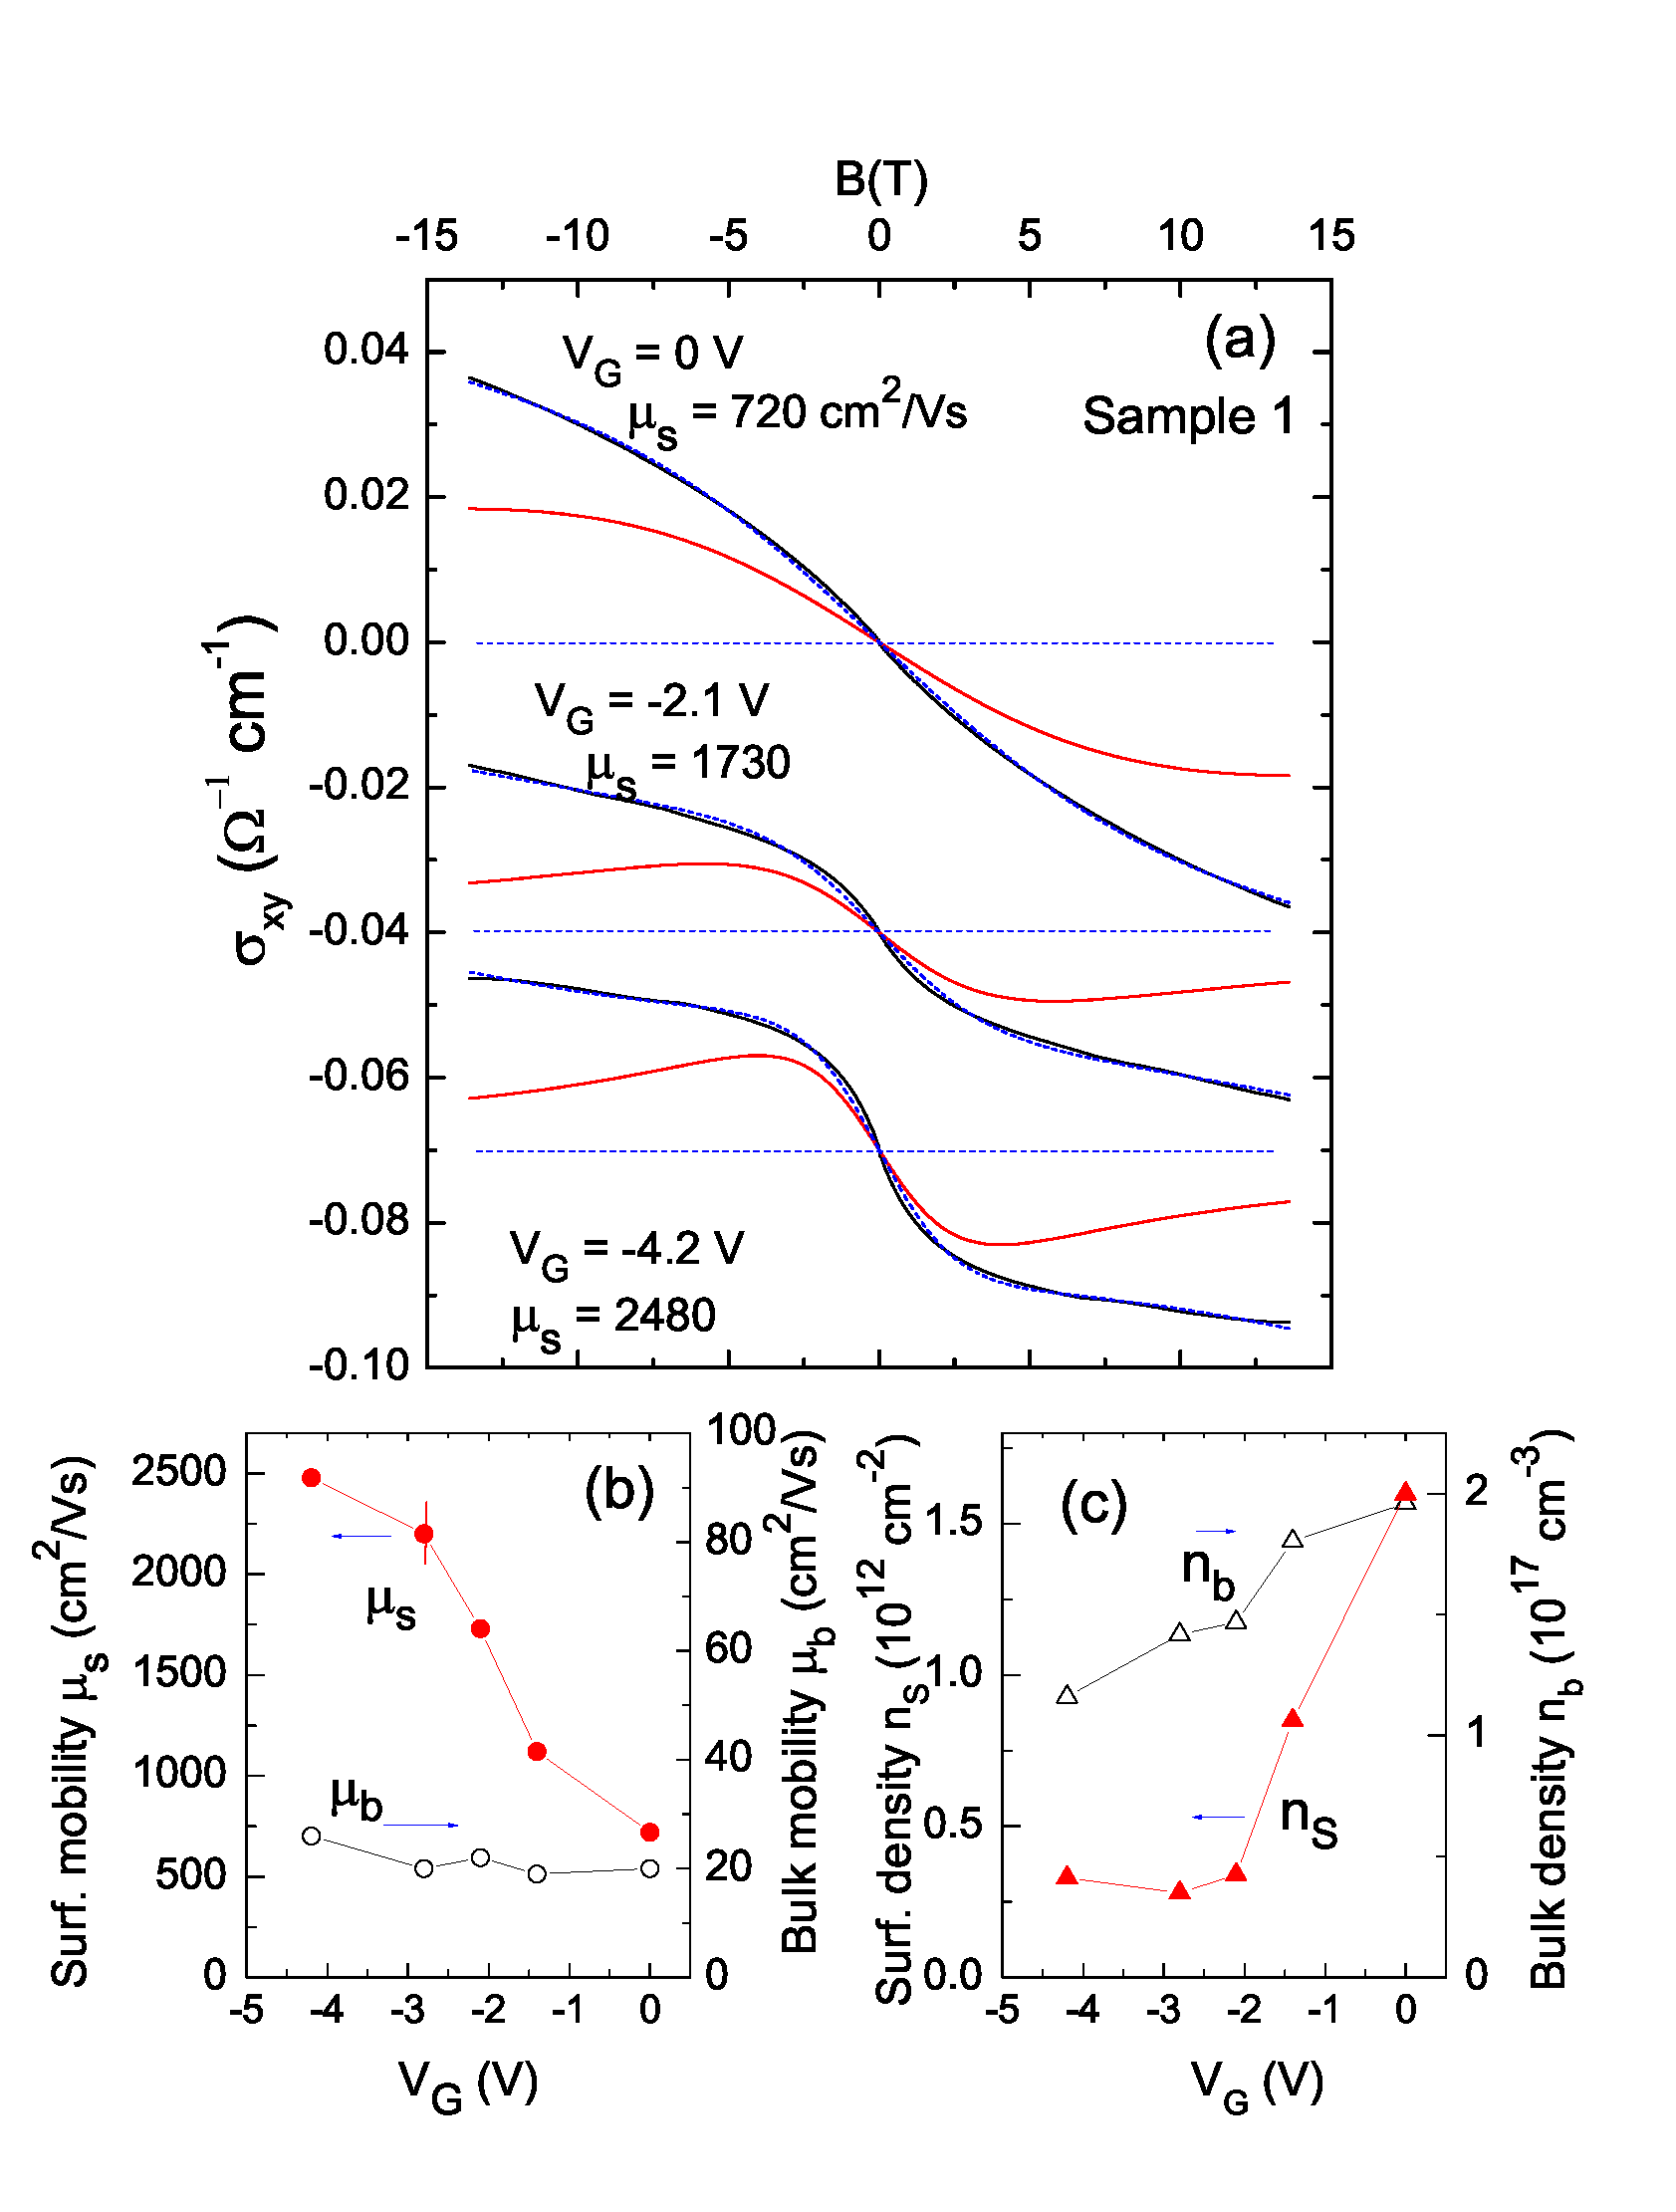
\includegraphics[width=0.85\linewidth]{ch-liquid/figures/FigHallMob3}
\caption{\label{figHall} (color online) 
Panel (a): The observed Hall conductivity $\sigma_{xy}$ vs. $B$ in Sample 1,
showing weak-$B$ curvatures at 3 values of $V_G$
(curves displaced for clarity). At each $V_G$, the outer curves are the 
data (solid black curve) and the fit to Eq. \ref{eq:sxy} (superposed blue dashed curve). The inner
(red, solid) curve is the surface term
$G^s_{xy}/t$ fixed by $n_s$ and $\mu_s$. (Weak SdH oscillations are apparent in the
observed $\sigma_{xy}$.) The difference 
between the outer and inner curves is the bulk term $\sigma^b_{xy}$. 
At $V_G$ = -4.2 V, $G^s_{xy}/t$ accounts for 83$\%$ of
$\sigma_{xy}$ in weak $B$. 
Panel (b) shows that, with increased gating, $\mu_s$ increases from 720 to 2,480 cm$^2$/Vs 
while $\mu_b$ stays very small (20-30 cm$^2$/Vs). Panel (c) 
compares the sharp decrease in $n_s$ with the mild change in $n_b$ with gating. When $|V_G|$ is larger than
2 V, $n_s$ saturates.
}
  \end{center}
\end{figure} 


The above analysis indicates the coexistence of high-mobility surface Dirac electrons and a larger population of bulk electrons in our Bi$_2$Te$_2$Se samples. Because of the 100-fold difference in mobilities,
the Dirac surface electrons account for 83$\%$ of the total weak-$B$ Hall conductance at large $|V_G|$. Since we only includes one surface in calculating the surface Hall conductance, and it already accounts for the majority of the total $\sigma_{xy}$. There is no room left for a comparably large $G^s_{xy}$ for the other surface. With the parameters above, we estimate that the Hall contribution from the other surface 
is less than 2$\%$ of $\sigma_{xy}$. It also implies a low mobility on the other surface ($\mu_s$ is $<$300 cm$^2$/Vs), which explains why we do not resolve the other surface in SdH oscillations.





%The large enhancement of $\mu_s$ (Fig. \ref{figHall}b)
%by the liquid gating method is perhaps the most intriguing 
%feature reported here. To our knowledge, this is the first realization of 
%enhancement of surface SdH amplitudes by an \emph{in situ} technique.%~\cite{mobility}
%A recent STM experiment~\cite{Beidenkopf2011} reveals that
%the Dirac Point closely follows spatial fluctuations of the local
%potential on length scales of 30-50 nm. This could lead to strong scattering
%of surface electrons. We speculate that, under liquid gating, the anions accumulate
%at local maxima in the potential, thereby levelling out the strongest spatial fluctuations.%~\cite{scatter}
%The results provide encouragement that alternative routes that even out local
%potential fluctuations can lead to further improvements in $\mu_s$.


\subsection{Depletion-layer Capacitance, Screening and Impurity Band}

Besides the information about the surface states, the above gating experiments can also provide us with quantitative results on the electronic parameters in the bulk depletion region. This is important because it yields detailed properties of the bulk and can guide future gating experiments. In particular, an advantage of our experiment is that the SdH oscillations fix both $n_s$ and $E_F$ of the surface carriers (hence the surface electrostatic potential $\varphi(0)$) at each applied $V_G$. Then we can combine it with the carrier density and conductivity of the bulk carriers, as well as the anion charge $Q$ accumulated on the crystal surface, to depict a detailed picture of the band-bending model and perform self-consistency checks in the depletion capacitance. We follow the standard analysis of field-effect gating as introduced in Ref.\cite{SternRMP,Ashcroft,Sze}. We also provide more details in the appendix. 

%Our main results are on the tuning of the SdH oscillations of the Dirac surface states. However, the 
%experiment also yields quantitative results on the electronic parameters in the depletion region,
%which provide detailed picture of what happens under liquid gating.
%A useful feature of the experiment is that, at each value of the applied gate voltage $V_G$, we can measure via the SdH oscillations
%both $n_s$ and $E_F$ of the surface carriers
%(hence the surface electrostatic potential $\varphi(0)$). In addition, we measure
%the carrier density and conductivity of the bulk carriers, and the anion charge $Q$ accumulated on the
%crystals surface. The 5 quantities provide a detailed picture of the
%band-bending process as well as self-consistency checks in determining the depletion capacitance. 
%We apply the standard analysis of field-effect gating~\cite{SternRMP,Ashcroft,Sze},
%which is summarized in Appendix \ref{appcap}. 

When the chemical potential lies inside the band gap at $V_G$=0 V, as in the case of Bi$_2$Te$_2$Se, the gating effect will induce band bending. Instead, if $E_F$ is high in the conduction band (as the case in as-grown Bi$_2$Se$_3$), the applied $\bf E$
leads to Thomas Fermi screening~\cite{Ashcroft} for which the screening length is
$\lambda_{TF} = \sqrt{\pi a_B/4k_F}$ is typically a few $\rm \AA$ ($a_B = \hbar^2/me^2$ is the Bohr radius).
If the impurity band is absent in the energy gap, a negative $V_G$ generates a depletion region at the surface of the sample.
However, in spite of a very large
bulk resistivity (2-6 $\Omega$cm) at 4 K, our current generation of Bi$_2$Te$_2$Se crystals still have a signifiant amount of bulk carriers ($n_b\sim$ 2$\times 10^{17}$ cm$^{-3}$). It indicates an impurity band that extends across the gap.
Nonetheless, the changes in the conductance in our gating experiments suggest that the band bending exists over a significant depletion region ($\sim$10 $\mu$m).
We will analyze this situation at the end of this section after we estimate the depletion capacitance.


At negative $V_G $, the electric field $\bf E$ from the anions on the sample surface repels bulk electrons away from the surface,
exposing the ionized donors within the depletion width $d$. 
In Figure \ref{figGate}a we show a sketch of the band bending near the surface exposed to the ionic liquid at $V_G$ $< $ 0 V.
As we explained in the ``Experimental Setup'' chapter, the ionic liquid polarizes to form two capacitors effectively when gated. Each capacitor has a spacing of the order of the molecular radius $a$. Both capacitors store the charge $Q$. 
The effective area $A'$ of the capacitor at the gate electrode is much larger than that of the capacitor at the crystal surface $A$. Thus most of the potential drop $V_G-V_s$ (between the gate and the sample surface) falls across the latter ($V_s$ is the voltage 
corresponding to $\varphi(0)$ at the surface and the ground is taken deep in the bulk at $x\to +\infty$) in Figure \ref{figGate}b.
In Sample 1, $A$ = 2.9 mm$^2$ and $A'$ = 30 mm$^2$. 
The $E$-field produced by the anion layer just to the left of the crystal surface is 
$E(0^-) = Q/A\epsilon_0$.


%%%%%%%%%%%%%%%%%%%%%%%%%%%%%%%%%%
%%%%%%%%%%%%%%%%%%%%%%%%%%%%%%%%%%
%%%%%%%%%%%%%%%%%%%%%%%%%%%%%%%%%% FIGURE 7
\begin{figure}[!htbp]
  \begin{center}
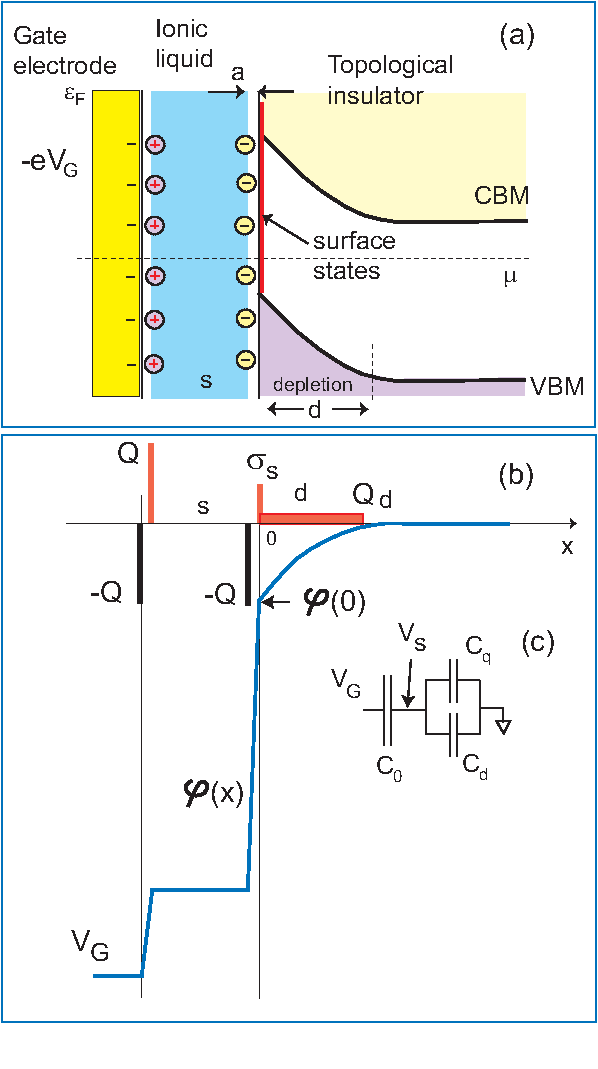
\includegraphics[width=0.65\linewidth]{ch-liquid/figures/FigGate.pdf}
\caption{\label{figGate} 
Sketch of band bending and the profiles of $\rho(x)$ and $\varphi(x)$ in the liquid gating experiment.
Panel (a) shows upwards bending of the bands induced by a negative gate voltage $V_G$. The cations and anions 
define two serial capacitors with spacing $a$ (molecular radius). The depletion layer in the bulk of the TI extends
a distance $d$. Panel (b) displays the charge distribution versus $x$. The negative charge $-Q$ on the gate electrode is
replicated by the anion layer separated by $a$ from the TI surface. This is compensated by the sum of the surface charge density
$\sigma_s$ and the ionized impurity charges inside the depletion layer. The electric potential $\varphi(x)$ corresponding to
$\rho(x)$ is sketched. Panel (c) shows the circuit of the equivalent capacitors $C_0$, $C_d$ and $C_q$.
}
  \end{center}
\end{figure} 



We also sketch the profiles of the charge density $\rho(x)$, the 
electrostatic potential $\varphi(x)$ (the $x$-axis is normal to the surface) and the effective capacitance configuration in Fig. \ref{figGate}b. 
The charge density $\rho(x)$ of the cations and anions in the ionic liquid can be regarded as
delta functions of strength $\pm Q$. In the TI sample, the surface charge density can also be represented by
a delta function ($\sigma_s$). Within the bulk, however, $\rho(x)$ is distributed 
over the depletion layer to a depth $d$. Here we adopt the usual approximation, 
where $\rho(x)$ is taken to be uniform for $0<x<d$. 
As a result, due to the uniform-charge approximation, $\varphi(x)$ varies as $-(x-d)^2$ in the depletion region.
At the surface $\varphi(0)$ becomes
\be
\varphi(0) = -N_ded^2/(2\epsilon_0\epsilon_s),
\label{phi0}
\ee
where $N_d$ is the donor impurity concentration and $\epsilon_s$ the screening dielectric parameter.
The charge $Q_d$ induced in the depletion width by $\varphi(0)$ defines the depletion capacitance
$C_d = N_dedA/\varphi(0) = \epsilon_0\epsilon_s A/d$. The surface charge density $\sigma_s$ 
induced by $\varphi(0)$ is represented by the quantum capacitance
$C_q = \sigma_s/\varphi(0) = e^2(dn_s/d\mu)$. Clearly, $C_d$ and $C_q$ are in parallel
combination (Fig. \ref{figGate}c).

The large slope change at $x=0$ mainly reflects the strong dielectric screening in the bulk of the
TI ($\sigma_s$ makes a negligible contribution). Thus the intense $E$-field produced by the
anions is strongly screened by polarization effects inside the crystal ($E(0^-)\gg E(0^+)$). 
As shown in Fig. \ref{figGate}c, the parallel combination of $C_d$ and $C_q$ is in 
series with $C_0$, the series combination of the cation and anion capacitances.
In all samples, we find that $C_d\gg C_q$, so we may ignore the quantum capacitance in the discussion below.

%\noindent
%\emph{Magnitude of $C_d$}\\
We analyze the magnitudes of the capacitors in Fig. \ref{RvsVG} as below. Fig. \ref{figIndexError}b shows that $E_F$ in Sample 1 decreases by $\sim$100 meV when the applied $V_G$ is -2 V.
Thus, most of the gate voltage drops in the liquid and only a small fraction ($\sim 1/20$) of the applied gate voltage is effective in bending the band ($V_s$ = -0.1 V).
Then we may estimate the depletion capacitance $C_d$ with the $C_0$, which could be assessed by the properties of the ionic liquid.
The value of $C_0/A$ for ionic liquids is approximately 11-12 $\mu$F/cm$^2$~\cite{Koch}.
It is obtained from the standard expression for capacitance, $C_0/A = \epsilon_0\epsilon_{liq}/a$, using $\epsilon_{liq}$ = 4, and $a$ = 3 $\rm\AA$. With the ratio $V_s/(V_G-V_s)\sim C_0/C_d$ (neglecting $C_q$), we estimate that $C_d/A\simeq$ 240 $\mu$F/cm$^2$.

Another method to estimate $C_d$ is by leveraging our observation of the charge flow in the gating experiment. As discussed in the appendix, we measure the ionic gating current when applying the gate voltage, and then integrate the ionic current over time to find the charge $Q$.
For Sample 1 with $V_G$ = -2 V, the ionic charge current deposits a total negative ionic charge at the surface equal to
$-Q/A\sim 2\times 10^{14}e$/cm$^2$ = -3.2$\times 10^{-5}$ C/cm$^2$. 
We notice that $Q/A$ is stored in $C_d$ by the voltage $V_s\sim$ 0.1 V,
so we have $C_d/A\sim$ 320 $\mu$F/cm$^2$, which is 33$\%$ larger than the first estimate. This error is still within our uncertainties since the inaccurate measurement of the actual area coated by the anions can provide the main source of the uncertainty. In our experimental setup, the ions can coat the silver paint contacts and voltage and current leads, and the area can exceeds that of the crystal $A$ by 50 to 100$\%$.

Using $\frac Q A = N_d e d + \sigma_s$, we can estimate the depletion width $d$ in our Bi$_2$Te$_2$Se crystal.
The donor density $N_d$ is roughly equal to the bulk density observed at 4 K, $n_b~\sim 2\times 10^{17}$ cm$^{-3}$.
This gives $d\simeq$ 10 $\mu$m, suggesting a thick depletion layer. We notice that the deep penetration of the depletion region into the bulk
is consistent (within a factor of 2) with the 40$\%$ change observed in the resistivity and Hall coefficient at 4 K.

From the range of $C_d/A$ (240-320 $\mu$F/cm$^2$), we find that the depletion capacitance in our Bi$_2$Te$_2$Se sample is 5,000-6,000$\times$ larger than the values commonly observed in a Si-MOSFET device ($C_{d,Si}/A\simeq$ 0.05-0.06 $\mu$F/cm$^2$~\cite{SternRMP,Sze}).
Such a giant enhancement in TI indicates a very large polarizability in its ground state when $E_F$ lies inside the energy gap. A possible underlying reason is the impurity band in Bi$_2$Te$_2$Se while energy gap in high-purity Si is devoid of impurity states. There is evidence for the impurity band in Bi$_2$Te$_2$Se in many experiments\cite{Ando10}. For example, the $\rho-T$ curve of
Bi$_2$Te$_2$Se at 4 K displays a small, but metallic conductivity possibly arising from a large population of impurity-band electrons.


In addition, we hope to make a comment on the finite DOS in the gap here.
In order to create an extended depletion region with significant band bending and a thick depletion layer, as we discuss above and show in Fig. \ref{figGate}a, 
the weak bulk conductivity must be further driven to zero throughout the depletion region
in order to sustain a finite $E$-field (otherwise one has Thomas-Fermi screening with the very short screening length 
$\lambda_{TF} \simeq$ 6 $\rm\AA$
for $n_b$ = 2$\times 10^{17}$ cm$^{-3}$m). This looks a little surprising at the first sight. But the existence of a mobility edge in the 
impurity band can explain how band-bending is sustained over a large depletion region without inducing the Thomas-Fermi screening. If $E_F$ lies below the mobility edge throughout the depletion layer,  then the bulk conductivity there will vanish at 4 K. Besides, because impurity-band states close to the mobility edge have a greatly enhanced polarizability in an $E$-field, we expect the electronic contribution to 
dielectric constant $\epsilon_s$ to be orders of magnitude larger than the lattice contribution. Our measurements of $C_d/A$ probe directly the electronic polarizability in the depletion region. We will discuss a possible scenario is described in the appendix.


\section{Discussion and Summary}
\label{sec:liquid:discussion}

We have tuned the $E_F$ of the surface Dirac fermions over a considerable range, by applying the novel ionic liquid gating technique to the insulating Bi$_2$Te$_2$Se crystals with $\rho >$ 4 $\Omega$cm at 5 K.
In contrast to previous gating experiments, we readily resolve prominent surface SdH oscillations 
at each gating voltage. From the SdH periods, we find that the surface Fermi energy $E_F$
(Sample 1) decreases  
from 180 mV to 75 mV above the Dirac Point as $V_G$ is changed from 0 to -2.8 V. 
In a 14 T magnetic field, the lower limit corresponds to
the middle of the broadened $N$ = 1 Landau Level. Attaining such low Landau levels enables the $-\frac12$
intercept (predicted for Dirac fermions) to be determined with high accuracy.
Furthermore, the intercepts are closely similar for a broad range of $V_G$ in both Samples 1 and 2, adding more evidence for a $\pi$ Berry phase of the surface Dirac electrons on Bi$_2$Te$_2$Se.

Through analyzing the SdH oscillations, we also obtain the surface mobility $\mu_s$ and density $n_s$ for the surface states. And our calculation shows that the Hall conductivity from the surface Dirac fermions exposed to the anions accounts
for up to 83$\%$ of the total observed weak-$B$ Hall conductivity at 5 K. Such a large proportion is mainly caused by the large difference between the surface and the bulk mobilities. Combining these parameters with a semi-classical two-band model, we obtain an accurate determination
of the bulk carrier mobility and density at each $V_G$ (Fig. \ref{figHall}). We find that the surface carrier density $n_s$ decreases steeply while the surface mobility
$\mu_s$ increases to a maximum value of 2,400 cm$^2$/(Vs) under gating. The bulk carriers are depleted to a depth of 10 $\mu$m from the 
surface, with $\mu_b$ remaining at the low value of 20 cm$^2$/(Vs).



The large enhancement of $\mu_s$
by liquid gating (Fig. \ref{figHall}b) is perhaps the most intriguing 
feature in our ionic liquid gating experiments. To our knowledge, this is the first realization of 
enhancement of surface SdH amplitudes by an \emph{in situ} technique, and may provide a way to improve the surface conductivity. A clue for the explanation arises from an STM experiment~\cite{Beidenkopf2011}, which reveals that
the Dirac Point closely follows spatial fluctuations of the local
potential on length scales of 30-50 nm. Such a large fluctuation in the surface band can lead to strong scattering
of surface electrons and then reduces the surface mobility. We speculate that, under liquid gating, the anions accumulate
at local maxima in the potential, thereby leveling out the strongest spatial fluctuations and improving the electron lifetime.
The results are encouraging and indicate that alternative routes that even out local
potential fluctuations can further improve $\mu_s$. This could be important for future applications and devices.

We also provide analysis and experimental data in order to uncover whether the ionic liquid gating actually alters the carrier concentration by chemical
reactions or simply through bending the band. 
By carefully selecting the experimental conditions (e.g. the gating temperature),
monitoring charge accumulated $Q$, and checking for reversibility, we establish that band-bending is the dominant effect
in our experiments. Lastly, the five quantities measured at each gate voltage setting ($E_F$, $n_s$, $n_b$, $\rho$ and $Q$)
provide a quantitative picture of the gating process and the band bending effect. The depletion
capacitance measured implies that, within the depletion region, the electronic polarizability is strongly enhanced.

